\documentclass[nochap]{apuntes}

\usepackage{tikztools}
\usepackage{fastbuild}

\usetikzlibrary{calc}

\precompileImages
\precompileTikz

\title{Geometría de curvas y superficies}
\author{Guillermo Julián Moreno}
\date{13 / 14 C2}

\begin{document}

\maketitle
\newpage
\pagestyle{plain}
\section{Introducción a curvas y superficies}

\subsection{Parametrización de curvas}
Existen varias formas de representar curvas en $\real^2$.

\begin{defn}[Curva\IS parametrizada diferenciable]
Es una aplicación diferenciable $\appl{\sigma}{I=(a,b)}{\real^n}$
\end{defn}

\begin{defn}[Velocidad\IS de una trayectoria] Dada una curva parametrizada de $ℝ^n$  $\appl{σ}{I}{ℝ^n}$, el vector velocidad de la trayectoria en $σ(t)$ es $σ'(t)$, su derivada.
\end{defn}

\begin{defn}[Rapidez\IS de una trayectoria] Dada una curva parametrizada de $ℝ^n$  $\appl{σ}{I}{ℝ^n}$, la rapidez de la trayectoria es $\md{σ'}$, el módulo de su derivada.
\end{defn}

Podemos tener varios \textit{accidentes} en una parametrización:

\begin{enumerate}
\item Que la parametrización no sea inyectiva.
\item Que sea inyectiva pero su inversa no sea continua.
\end{enumerate}

Por lo tanto, buscaremos un tipo de parametrizaciones \textit{buenas}:

\begin{defn}[Parametrización\IS bicontinua] Se dice que una parametrización es bicontinua si ella y su inversa son continuas.
\end{defn}

Por la propia definición, una parametrización regular es localmente bicontinua.

\begin{defn}[Longitud\IS de arco] Sea $\appl{σ}{(a,b)}{ℝ^N}$ una trayectoria de clase $C^1$. Entonces la longitud de arco de σ está definida por

\[ L(σ) = \int_a^b \md{σ'(t)} \dif t \]
\end{defn}

La longitud de arco nos permite definir una parametrización para cualquier curva:

\begin{defn}[Parametrización\IS por longitud de arco] Se dice que una curva $\appl{σ}{I}{ℝ^n}$ está parametrizada por longitud de arco si $\md{σ'(s)} = 1\;\forall s∈I$.
\end{defn}

Igualmente, también querremos crear una reparametrización que nos lleve una parametrización regular cualquiera a una parametrización por longitud de arco.

\begin{prop} Para toda curva parametrizada regular $\appl{σ}{I}{ℝ^N}$ existe una transformación de parámetros que conserva la orientación , $h$, tal que $σ○h$ está parametrizada por longitud de arco.
\end{prop}

\begin{proof} Para reparametrizar, buscamos cambiar cómo nos movemos por el parámetro sin variar el conjunto imagen en $ℝ^3$, según el esquema de \ref{figParamLongArco}.

\begin{wrapfigure}{r}{0.4\textwidth}
\centering
\begin{tikzpicture}
\node (I) at (0,0) {$t∈I⊆ℝ$};
\node (J) at (0,-3) {$s∈J⊆ℝ$};
\node (R) at (3,0) {$ℝ^N$};

\draw[->] (J) -- node[left] {$f$} (I);
\draw[->] (I) -- node[above] {$σ$} (R);
\draw[->] (J) -- node[below right] {$β=σ○f$} (R);
\end{tikzpicture}
\caption{Reparametrización por longitud de arco.}
\label{figParamLongArco}
\end{wrapfigure}

Buscamos que $f$ sea un difeomorfismo (esto es, que exista su inversa y que sea diferenciable).

La reparametrización por arco de $σ$ es la aplicación $β(s)$ construida como en (\ref{figParamLongArco}) tal que $\md{β'(s)}=1$.

Sabemos que

\[ β'(s) = \deriv{β}{s}(s) = \deriv{σ}{t}(f(s))\cdot \deriv{f}{s}(s) \]

y por lo tanto
\[ \abs{f'(s)} = \frac{1}{\md{α'(f(s))}} \]

Entonces necesitamos que $σ'(t)≠0\; ∀t∈I$ (que sea regular). Además, si $f(s)$ es creciente

\[ f'(s) = t'(s) = \frac{1}{\md{σ'(t(s)}} \implies s'(t) = \md{σ'(t)} \]

y nos quedaría

\[ s(t) = \int_{t_0}^t \md{σ'(t)}\dif t \]

que es la reparametrización que buscamos.

\end{proof}

\begin{lemma} Sean $\appl{σ_1}{I_1}{ℝ^N}$, $\appl{σ_2}{I_2}{ℝ^N}$ dos parametrizaciones por arco de la misma curva. Entonces la transformación de parámetros correspondiente $\appl{h}{I_1}{I_2}$ tal que $σ_1=σ_2○h$ es de la forma \[ h(s) = \pm s + s_0 \] con $s_0∈ℝ$ constante.

$s$ será positivo si la orientación es compatible y negativa si la orientación de ambas parametrizaciones es opuesta.

En otras palabras: dos parametrizaciones por arco sólo se distinguen en el punto inicial ($s_0$) y en la dirección en la que recorren la curva.
\end{lemma}

\begin{proof} Sabemos que

\[ 1 = \md{σ_1'(s)} = \md{(σ_2○h)'(s)} = \md{σ_2'(h(s))\cdot h'(s)} = \md{σ_2'(h(s))} ·  \abs{h'(s)} = \abs{h'(s)} \]

Integrando $\abs{h'(s)}$ nos queda que $h(s) = \pm s + s_0$.
\end{proof}

\paragraph{Método para reparametrizar por arco} Partimos de una curva cualquiera $α(t)$, y queremos reparametrizarla por arco, esto es, buscamos una función $t(s)$ tal que $α(t(s))$ sea PPA. Nuestro nuevo parámetro es entonces

\[ s(t) = \int_{t_0}^t \md{α'(x)}\dif x \]

donde $t_0$ es un punto inicial totalmente arbitrario. Ahora bien, nosotros buscamos $t(s)$, así que invertimos la función $s$. Por ejemplo, si la integral nos hubiese dado

\[ s(t) = \cos t \]

la inversa sería

\[ t(s) = \arccos s \].

Ahora sustituimos en nuestra curva las $t$ por $t(s)$. Si por ejemplo nuestra curva fuese $α(t) = (t, e^t)$ y tomamos $t(s)$ lo que nos ha dado antes, tendríamos que nuestra curva PPA sería
\[ α(t(s)) = (\arccos s, e^{\arccos s}) \]

\section{Curvas planas}

\begin{defn}[Curvatura] Dada una curva regular en $ℝ^N$, el campo \mv{k} de los vectores curvatura de la misma es el formado por la derivada segunda $β''(s)$, siendo β una parametrización por longitud de arco.
\end{defn}

De forma trivial, se verifica que la derivada segunda \textbf{no depende de la parametrización} por arco elegida.

Si además consideramos el campo \mv{t} de las tangentes unitarias de la curva\footnote{$\displaystyle\mv t(s) = \frac{α'(s)}{\md{α'(s)}}$}, tenemos que, independientemente de la parametrización:

\[ \mv k(s) \equiv α''(s) \equiv \mv t'(s) \]

Esto nos lleva a una primera propiedad interesante de la curvatura:

\begin{lemma} Dada una curva regular en $ℝ^N$, su vector curvatura es normal a la curva en cada punto
\end{lemma}

Por otra parte, la curvatura cumple una idea muy sencilla: si su valor es 0, estamos ante una recta. Dicho de otra forma:

\begin{lemma} Una curva regular en $ℝ^N$ es un trozo de recta afín si y sólo si $\mv k = 0$. \end{lemma}

\par

Hasta ahora hemos tratado la curvatura sobre parametrizaciones por longitud de arco. ¿Cómo podemos obtenerla si estamos tratando con cualquier otro parámetro α?

Sabemos que podemos escribir una reparametrización de α, así que podemos efectivamente "normalizar" la curvatura y el campo de tangentes:

\begin{gather*}
\mv t(s) = \frac{α'(s)}{\md{α'(s)}} \\
\mv k(s) = \frac{α''(s)}{\md{α'(s)}^2} - \left(\mv t \frac{α''(s)}{\md{α'(s)}^2}\right) \mv t
\end{gather*}

En el caso de \mv{k}, lo que hacemos es quitarle a la normalización la componente tangencial, la que tiene la misma dirección que \mv{t}.\footnote{A grandes rasgos, esto equivale a aplicar la ortogonalización de Gram-Schmidt al par de vectores $\displaystyle\left\{\mv t, \frac{α''(s)}{\md{α'(s)}^2}\right\}$.}

A partir del vector curvatura, podemos definir el vector normal unitario $\cn$ como la rotación por 90º de $\ct$. $\cvv$ es proporcional a ese vector unitario, y de hecho

\[ \cvv = \cv \cn \]

con $\cv$ la curvatura escalar. La curvatura escalar se puede obtener también como

\[ k(t) = \cn \cv = \det [\ct | \cvv ] = \det \begin{pmatrix}
t_0 & k_0 \\
t_1 & k_1
\end{pmatrix} \]

\subsection{Círculo osculador y curva evoluta}

\begin{defn}[Círculo\IS osculador] Se define el círculo osculador de una curva α en un punto $p=α(t_0)$ a la circunferencia tangente a α en $p$ con curvatura $\cv[α](t_0)$.
\end{defn}

Si trazamos la trayectoria de los centros de los círculos osculadores, llegamos a la curva evoluta:

\begin{defn}[Evoluta] La curva evoluta de una curva α se define como

\[ β(t) = α(t) + \frac{1}{\cv(t)}\cn(t) \].

Además, la curva evoluta es la envolvente a las rectas normales a la curva α en todos sus puntos. Ver figura \ref{imgEvoluta}.
\end{defn}

\easyimg{img/Evoluta.png}{La curva evoluta es el conjunto de todos los centros (naranjas) de los círculos osculadores (verde). Además, todas las rectas normales a la curva (gris) envuelven la evoluta.}{imgEvoluta}

\subsection{Reconstrucción a partir de una función de curvatura} Dada una función suave $\appl{k}{I}{ℝ}$, las curvas que tienen $k$ como función de curvatura se construyen como

\[ θ(s) = \int k(s) \dif s + θ_0 \]

de tal forma que

\[ \left.\begin{matrix}
x'(s) = \cos θ(s) \\
y'(s) = \sin θ(s)
\end{matrix}\right\} \implies
\begin{matrix}
x(s) = \int\cos θ(s)\dif s + x_0 \\
y(s) = \int \sin θ(s) \dif s + y_0
\end{matrix} \]

Así reconstruimos la curva salvo un movimiento rígido (giro o traslación).

Además, dadas dos curvas PPA, $\appl{α,b}{I}{ℝ^2}$ con la misma curvatura escalar $k_α=k_β$, entonces existe un único movimiento rígido $M$ de $ℝ^2$ que preserva orientación, tal que

\[ β(s) = M ○ α(s)\; ∀s∈I \]

\subsection{Diedro de Frenet}

Partimos de una curva $\appl{α}{I}{ℝ^2}$, parametrizable por arco con $α=α(s)$. De ella podemos obtener el \textbf{diedro de Frenet}, una base ortonomal del plano dada por

\[ \mv{t}_{α} = α'(s);\quad \mv{n}_α(s) = R_{\frac{π}{2}} \mv{t} (s) \]

donde $R_{β}$ es una rotación por un ángulo β.

Podemos considerar el producto escalar $\pesc{\mv{n}_α(s),\mv{n}_α(s)}$ que es igual a 1  (el vector normal es unitario). Podemos derivar, y nos queda

\[ 0 = 2\pesc{\mv{n}'_α(s), \mv{n}_α(s)} \]

Por lo tanto, la tangente al normal es perpendicular al normal. La cuestión es encontrar ahora la relación entre sus módulos. Para ello derivamos el producto escalar del vector normal y del tangente:

\[0 = \pesc{\mv{n}_α,\mv{t}_α}' = \pesc{\mv{n}_α', \mv{t}_α} + \pesc{\mv{n}_α, \mv{t}_α'} = \stackrel{\text{Ec. Frenet}}{=} \pesc{\mv{n}_α', \mv{t}_α} + \pesc{\mv{n}_α,k_α\mv{n}_α} \]

y entonces

\[ \pesc{\mv{n}_α', \mv{t}_α} = -k_α(s) \]

Con la base ortonormal del diedro de Frenet podemos escribir un vector $\vu$ como

\[ \vu = \pesc{\vu, \mv{t}_α(s)}\mv{t}_α(s) + \pesc{\vu, \mv{n}_α(s)}\mv{n}_α(s)\]

y por lo tanto podemos reescribir

\[ \mv{n}' = \underbrace{\pesc{\mv{n}', \mv{t}_α(s)}}_{-k_α(s)} \mv{t}_α(s) + \underbrace{\pesc{\mv{n}', \mv{n}_α(s)}}_{0}\mv{n}_α(s)\]


\section{Curvas en el espacio}

Tal y como hacíamos en curvas en el plano, en el espacio partimos del triedro de Frenet\index{Triedro!de Frenet}. Además de los vectores tangente $\ct$ y normal $\cn$, tendremos el vector binormal:

\[ \cb = \ct × \cn \]

de tal forma que $\{\ct,\cn,\cb\}$ es una base del espacio $ℝ^3$. Además, $\{\ct,\cn\}$ es una base del \textbf{plano osculador}\index{Plano!osculador}.

El tiedro de Frenet satisface el siguiente sistema:

\[ \begin{matrix}
\ct'(s) &= & & k\cn & \\
\cn'(s) &= & -k\ct & + & \ctr \cb \\
\cb'(s) &= & & -\ctr \cn &
\end{matrix} \]

donde τ es la torsión, que nos da una medida de lo \textit{no plana} que es la curva. De hecho, si $τ = 0$, la curva es plana.

\begin{defn}[Curva\IS birregular] Se dice que una curva $\appl{α}{I}{ℝ^3}$ es birregular si $α'(t)$ y $α''(t)$ son linealmente independientes (no se anulan) para todo $t∈I$.
\end{defn}

\section{Superficies: primera forma fundamental}

En esta sección vamos a pasar a estudiar las superficies en el espacio, más concretamente las superficies suaves o regulares.

\begin{defn}[Superficie\IS suave]\index{Superficie!regular} Dada una parametrización $\appl{Φ(u,v)}{A⊆ℝ^2}{ℝ^n}$ de una superficie, se dice que es regular si el vector normal no es nunca cero. Esto es, \[ Φ_u(u,v) × Φ_v(u,v) ≠ 0 \quad ∀(u,v) ∈ A \]. Dicho de otra forma, Φ tiene que ser un difeomorfismo.
\end{defn}

Una forma familiar de parametrizar las superficies es a través de rectas (generatrices) que se mueven a lo largo de una curva directriz. Por ejemplo, un cono es una \concept{superficie\IS reglada}: lo generamos con las rectas entre un punto fijo y todos los puntos de una circunferencia (la curva directriz).

Podemos materializar esta idea en una ecuación, una representación paramétrica de una superficie reglada:

\[ Φ(t,u) = p(t) + u·r(t) \], donde $p$ sería la parametrización de la curva directriz y $r$ el vector director de la recta en cada punto.

\begin{figure}[hbtp]
\centering
\inputtikz{SuperficieReglada}
\label{imgSuperficieReglada}
\caption{Podemos reglar la silla usando dos familias de rectas distintas}
\end{figure}

En algunos casos las superficies se pueden reglar de dos maneras diferentes. Por ejemplo, la silla $z=xy$ (imagen \ref{imgSuperficieReglada}) se puede reglar de dos formas distintas, ya sea con las rectas paralelas al eje $X$ o con las paralelas al eje $Y$.

¿Qué vamos a querer hacer en las superficies? Lo normal será medir la longitud de curvas en la superficie, encontrar el área de regiones de la superficie o ver el ángulo entre dos curvas.

Para esas tareas, en el espacio usamos el producto escalar. Necesitamos generalizar este concepto para las superficies, y para ello recurrimos a las métricas.

\begin{defn}[Métrica\IS Riemanniana] La métrica riemmaniana de una superficie $S$ en un punto $p$ se define como una aplicación suave $\appl{Q}{T_pS×T_pS}{ℝ}$ definida positiva\footnote{$Q$ es definida positiva si $Q(\vu, \vv) > 0\quad ∀(\vu,\vv)≠(\vec{0},\vec{0}) ∈ T_pS×T_pS$.}\end{defn}

La métrica $Q$ nos da, para cada punto $p∈S$, una \textit{forma de medir}, una especie de producto escalar que podemos aplicar a los vectores tangentes a la superficie en ese mismo punto.

Ahora necesitamos encontrar una métrica para cada superficie $S$ parametrizada por la aplicación $Φ(u,v)$. Hemos dicho que es un producto escalar, así que vamos a calcular cuál es el producto escalar de dos vectores cualquiera $\va,\vb$ que pertenezcan al espacio tangente de $S$.

Recordemos que el espacio tangente tiene como base los vectores $\pd{Φ}{u}=Φ_u$ y $\pd{Φ}{v} = Φ_v$. Por lo tanto, podemos reescribir $\va = a_1Φ_u + a_2Φ_v$ y $\vb = b_1Φ_u + b_2Φ_v$. Si calculamos su producto escalar:
\begin{align*}
\pesc{\va, \vb} &= \pesc{a_1Φ_u + a_2Φ_v, b_1Φ_u+b_2Φ_v} = \\
	&= a_1b_1 \pesc{Φ_u, Φ_u} + (a_1b_2 + a_2b_1) \pesc{Φ_u,Φ_v} + a_2b_2\pesc{Φ_v, Φ_v} = \\
	&= a_1b_1E + (a_1b_2 + a_2b_1) F +  a_2b_2G
\end{align*}

Esta métrica, que hemos hallado a partir del producto escalar euclídeo, se llama la \textbf{primera forma fundamental}\index{Primera forma fundamental}, denotada como $I_Φ$ y comprime todas las propiedades métricas de la superficie. Otra forma de expresarla sería como una matriz simétrica:

\[ I_Φ (\va, \vb) = \va^T \begin{pmatrix} E & F \\ F & G \end{pmatrix} \vb \]

Recordemos que los coeficientes se hallan a partir de las derivadas de la parametrización:
\begin{align*}
E &= \pesc{Φ_u, Φ_u} \\
F &= \pesc{Φ_u,Φ_v} \\
G &= \pesc{Φ_v, Φ_v}
\end{align*}

A partir de la primera forma fundamental, podemos expresar el elemento de línea como \[\dif s^2 = E\dif u^2 + 2F\dif u\dif v + G\dif v^2\], lo que nos permite calcular la longitud de una curva $(u(t), v(t))$ en la superficie \[ L = \int_I \sqrt{ E\left(\od{u}{t}\right)^2 + 2F\od{u}{t}\od{v}{t} + G\left(\od{v}{t}\right)^2 } \dif t \] y el área de una región $M⊆S$:

\[  A = \iint\limits_M \sqrt{EG-F^2} \dif u \dif v \]

\subsection{Isometrías}

Una vez que ya sabemos medir en superficies, nos interesará ver si dos superficies tienen una estructura similar en este sentido, esto es, si son isométricas.

\begin{defn}[Isometría\IS local] Sean $S,M$ dos superficies. Se dice que $\appl{h}{S}{M}$ es una isometría local si es $C^1$ y conserva las distancias. Esto es, dada una función distancia $d_S$ y $d_M$ para ambas superficies respectivamente, se tiene que

\[ d_S(a,b) = d_M(h(a), h(b)) \]
\end{defn}

\begin{defn}[Isometría\IS global] Una aplicación $\appl{h}{S}{M}$ es global si además de ser isometría local es aplicación biyectiva. \end{defn}

Una propiedad interesante de las isometrías es su relación con la primera forma fundamental. Habíamos dicho que la primera forma fundamental es la manera que tenemos de medir distancias en la superficie, por lo que si la isometría conserva las distancias la primera forma fundamental también habría de conservarse, ¿no? Formalicémoslo.

\begin{theorem} Dadas dos parametrizaciones $\appl{Φ}{A⊆ℝ^2}{S}$ y $\appl{Ψ}{A⊆ℝ^2}{M}$ de las respectivas superficies $S$ y $M$, definidas en el mismo dominio $A$, consideramos una aplicación suave \begin{align*}\appl{h}{S&}{M} \\ Φ(u,v) &\xrightarrow{h} Ψ(u,v) \end{align*}

Entonces, $h$ es una isometría si y sólo si $I_Φ \equiv I_Ψ$, esto es, se conservan los coeficientes de la primera forma fundamental.
\end{theorem}

\section{Curvatura de superficies: Segunda forma fundamental}

Hasta ahora hemos visto cómo medir en superficies. Sin embargo, el estudio de estos objetos no se queda ahí. También querremos saber cómo de curvadas están, y esta es la motivación para introducir varios conceptos. El primero es de la curvatura normal, que nos indica \textit{cuánto} se separa la superficie de su plano tangente. Una curvatura normal pequeña nos indicará una superficie más cercana al plano tangente, mientras que si es muy grande nos indica que en ese punto la superficie es uy curvada.

Por simplificar, asociaremos la curvatura normal a una curva en la superficie.

\begin{defn}[Aceleración\IS normal] Dado un campo normal unitario $N$ de la superficie $S$, definimos la aceleración normal de α en $S$ como
\[ a_α(t) = α''(t) \cdot N_{α(t)}\]
\end{defn}

\begin{defn}[Curvatura\IS normal] Dado un campo normal unitario $N$ de la superficie $S$, definimos la curvatura normal de α en $S$ como

\[ k_{α,n}(t) = N_{α(t)} \cdot \cv(t) \]
\end{defn}

Es decir, la curvatura normal es la componente del vector curvatura de la curva normal a la superficie. Si tenemos la suerte de que α sea PPA, tenemos que $\cv(t) \equiv α''(t)$, y la aceleración normal y la curvatura normal coinciden.

\subsection{Endomorfismo de Weingarten y segunda forma fundamental}

\begin{wrapfigure}{r}{0.4\textwidth}
\centering
\inputtikz{BalanceoNormal}
\caption{La normal se balancea a un lado y a otro a lo largo de la superficie (en este caso, una sección de ella)}
\label{imgBalanceo}
\end{wrapfigure}

El endomorfismo de Weingarten y la segunda forma fundamental surgen de manera natural al estudiar cómo se curvan las superficies. Para ello, nos fijaremos en cómo se balancea el vector normal (figura \ref{imgBalanceo}).

Vamos a empezar con nuestra superficie $M$ y un punto $p∈ M$. Consideramos un entorno $W$ del punto $p$. Sea $\appl{n}{W}{ℝ^3}$ la aplicación que lleva cada punto de $W$ a su correspondiente vector normal unitario. Queremos ver cuánto varía el vector normal y hacia dónde en ese entorno, así que introducimos la noción de derivada direccional:

\begin{defn}[Derivada\IS direccional] Dada una aplicación $\appl{f}{S}{ℝ^3}$, la derivada de $f$ en la dirección $\vv$ en $\va$ (notación: $\Dif_{\vv} f(\va)$) se define como la derivada de $f○α$, con α una curva tal que $α(0) = p$ y $α'(0) = \vv$, en $t=0$.
\end{defn}

De aquí podemos sacar el endomorfismo de Weingarten, también llamado \textbf{operador de forma}\index{Operador!de forma}, que nos indica cómo varía el vector normal en una dirección determinada.

\begin{defn}[Endomorfismo\IS de Weingarten] Definimos la aplicación \textbf{lineal} de Weingarten para una superficie $S$ en un punto $p$ como $\appl{\wein}{T_pS}{T_pS}$, dada por \[ \wein(\vx) = - \Dif_{\vx} \vn \] con $\vn$ el vector normal a $S$ en $p$.
\end{defn}

Esto es, el vector $\wein(\vx)$ nos dice hacia dónde varía el vector normal cuando nos movemos en la superficie en la dirección $\vx$ desde el punto $p$, tal y como se ve en la figura \ref{imgWeingarten}. Se puede demostrar que la aplicación es en efecto un endomorfismo, y que $∀\vx ∈ T_pS \quad \wein(\vx) ∈ T_pS$ mostrando que sigue siendo ortogonal al vector normal.

\begin{figure}[hbtp]
\centering
\inputtikz{Weingarten}
\label{imgWeingarten}
\caption{Representación del endomorfismo de Weingarten: es la variación del vector normal en la dirección dada (es decir, a lo largo de una curva σ con $σ'(0) = \vv$).}
\end{figure}

Partiendo del endomorfismo de Weingarten llegamos a la segunda forma fundamental:

\begin{defn}[Segunda forma fundamental][Forma fundamental!segunda] Dada una superficie $S$ por una parametrización $Φ(u,v)$, denotamos la segunda forma fundamental como \[ II_Φ(\vv) = \pesc{\wein(\vv), \vv} = e \dif u^2 + 2 f \dif u \dif v + g \dif v^2 =
\vv^T · \begin{pmatrix} e & f \\ f & g\end{pmatrix} · \vv\], con \begin{align*}
e &= \pesc{\vn, Φ_{uu}} \\
f &= \pesc{\vn, Φ_{uv}} \\
g &= \pesc{\vn, Φ_{vv}}
\end{align*}

Recordamos que el producto escalar que estamos usando es el definido por la métrica, es decir, por la primera forma fundamental. Por lo tanto, $\pesc{\wein(\vv), \vv} = I(\wein(\vv), \vv)$.
\end{defn}

La segunda forma fundamental evaluada en $\vv$ nos da una \textit{medida} de cuánto varía el vector normal en la dirección de $\vv$ al movernos hacía ahí. Cuanto mayor sea, mayor será la variación del vector normal en la dirección de $\vv$ y por lo tanto mayor la curvatura de la superficie. Si operamos con el vector tangente de una curva $α$, tenemos que \[ II_Φ(α') = α'' \].

\begin{proof}
Sabemos que $∀s$ a lo largo de α,  $\pesc{α', n ○ α} = 0$. Derivando, \[ 0 = \pesc{α', \vn ○ α}' = \pesc{α'', \vn ○α} + \pesc{α', (\vn ○α)'} \]. Cuando $s=0$, tenemos que

\begin{align*}
\pesc{α'', \vn} + \pesc{\ct, \Dif_{\ct} \vn} &= 0 \\
\pesc{α'', \vn} &= - \pesc{\ct, \wein(\ct)} \\
k_n &= II(\ct)
\end{align*}
\end{proof}

Antes de seguir, tenemos que ver de dónde vienen los coeficientes $e,f,g$ de la segunda forma fundamental. Sabemos que $II$ es una forma cuadrática, por lo que viene dada por la matriz

\[ II(\vv) = \vv^T \begin{pmatrix} e & f \\ f & g\end{pmatrix}  \vv \] en la base $\{Φ_u, Φ_v\}$. Para saber cuánto valen, operamos con los vectores $Φ_u$ y $Φ_v$, que en la base que consideramos son $(1,0)$ y $(0,1)$ respectivamente:

\begin{align*}
II((1,0)) &= \begin{pmatrix}1 & 0\end{pmatrix} \begin{pmatrix} e & f \\ f & g\end{pmatrix}\begin{pmatrix}1 \\ 0\end{pmatrix} = e \\
II((0,1)) &= \begin{pmatrix}0 & 1\end{pmatrix} \begin{pmatrix} e & f \\ f & g\end{pmatrix}\begin{pmatrix}0 \\ 1\end{pmatrix} = g \\
\end{align*}

Hallamos $f$ como $II((1,0), (0,1))$. Centrémonos en el primer caso, $II((1,0))$. La segunda forma fundamental está definida a partir de \wein, por lo tanto

\[ e = II((1,0)) = \pesc{\wein(Φ_u), Φ_u} = \pesc{\vn_u, Φ_u} \] donde $\vn_u = - \Dif_u \vn$. ¿Cómo hallamos ese valor? Podemos partir de que $\pesc{\vn, Φ_u} = 0$ y a partir de ahí derivar con respecto a $u$ otra vez:

\begin{align*}
\pesc{\vn, Φ_u}' &= 0 \\
- \pesc{\vn_u, Φ_u} + \pesc{\vn, Φ_{uu}} &= 0 \\
\pesc{\vn_u,Φ_u} &= \pesc{\vn, Φ_{uu}}
\end{align*}

Análogamente obtenemos los coeficientes para $f$ y $g$.

\subsection{Curvaturas}

Nos interesa el estudio de dos curvaturas, las \concept[Curvatura!principal]{curvaturas principales} a las que llamaremos $κ_1$ y $κ_2$, que se definirán respectivamente como

\begin{align*}
κ_1 &= \max_{\md{\vv} = 1} II(\vv) \\
κ_2 &= \min_{\md{\vv} = 1} II(\vv) \\
\end{align*}

Sin embargo, así visto es difícil calcular esas dos curvaturas. Vamos a usar algo de álgebra lineal, aprovechando que $II$ es una aplicación autoadjunta.

\begin{defn}[Aplicación\IS autoadjunta] Una aplicación $\appl{A}{V}{V}$ de un espacio vectorial en sí mismo es autoadjunta con el producto escalar $\pesc{·,·}$ si se cumple que, $∀\va, \vb ∈ V$ \[\pesc{A\va, \vb} = \pesc{\va, A\vb} \]
\end{defn}

\begin{theorem}[Teorema\IS espectral] Dada $A$ una aplicación autoadjunta en $ℝ^N$, todos sus autovalores son reales.
\end{theorem}

\begin{proof}(\href{http://www.proofwiki.org/wiki/Eigenvalues_of_Self-Adjoint_Operator_are_Real}{Fuente}) Si $A$ es una matriz real de dimensión $n$, ya sabemos que tiene $n$ autovalores, que no tienen por qué ser reales. Supongamos que $λ$ es una autovalor de $A$ asociado al autovector $\vv$. Entonces

\[ λ\pesc{\vv, \vv} = \pesc{λ\vv, \vv} = \pesc{A\vv, \vv} = \pesc{\vv, A\vv} \]

Usando la propiedad de simetría conjugada del producto escalar, nos queda \[ \pesc{\vv, A\vv} = \conj{\pesc{A\vv, \vv}} = \conj{\pesc{λ\vv, \vv}} = \conj{λ}\pesc{\vv, \vv} \] luego $λ=\conj{λ}$. Es decir, λ es un autovalor real.
\end{proof}

El Teorema espectral nos dice que habrá por lo tanto una base ortonormal de autovectores con autovalores reales asociados para el endomorfismo de Weingarten $\wein$. Con esta información podemos\footnote{Esto está basado en el \href{http://math.mit.edu/~stevenj/18.303/minmax.pdf}{teorema Min-Max}.} operar sobre $II(\vv)$.

Si $\{\ve_1, \ve_e\}$ es una base de autovectores normales asociados a los autovalores $\{λ_1, λ_2\}$ con $λ_1 ≥ λ_2$, podemos descomponer $\vv = a \ve_1 + b \ve_2$. Entonces, usando que $\wein$ es una aplicación bilineal,

\[ \wein(\vv) = \wein(a \ve_1 + b \ve_2) = \wein(a \ve_1) + \wein(b \ve_2) = aλ_1\ve_1 + bλ_2\ve_2 \]

Con esta información, podemos calcular $II(\vv)$:

\[ II(\vv) = \pesc{\wein{\vv}, \vv} = \pesc{aλ_1\ve_1 + bλ_2\ve_2, a \ve_1 + b \ve_2} = a^2λ_1 + b^2λ_2
\]
ya que, si la base es ortonormal, $\pesc{\ve_1, \ve_2} = 0$.

Si consideramos los vectores con módulo 1, $a^2 + b^2=1$ y entonces podemos acotar \[ a^2λ_1 + b^2λ_2 ≥ a^2λ_1 + b^2λ_1 = λ_1 \], y de forma análoga con $λ_2$. Esto es, los autovalores acotan por ambos extremos el valor de $II(\vv)$ con $\md{\vv} = 1$, luego son las curvaturas principales que buscábamos.

Puede darse el caso de que ambas curvaturas principales sean iguales. Denotaremos puntos de este tipo como \concept[Punto!umbilical]{puntos umbilicales}.

A partir de aquí definimos la curvatura más definitoria de una superficie: la curvatura gaussiana\footnote{
También se puede definir la curvatura media como la media de ambas curvaturas, pero todavía no sé para qué puñetas se usa, así que voy a pasar por encima.}

\begin{defn}[Curvatura\IS gaussiana] Dada una superficie $S$ con curvaturas principales $κ_1,κ_2$, se define la curvatura gaussiana como \[ K = κ_1κ_2 \], que también se puede expresar en función del determinante del operador de forma o endomorfismo de Weingarten:

\[ K = \det \wein \]
\end{defn}

El problema que tenemos ahora es hallar la matriz del endomorfismo de Weingarten \wein. Para ello simplemente operamos de forma matricial. Por un lado, \[ II(\vv) = \vv^T \begin{pmatrix}e & f \\ f & g\end{pmatrix} \vv \]. Por otro, \[ II(\vv) = \pesc{\wein(\vv), \vv} = \pesc{\vv, \wein(\vv)} = I(\vv, \wein(\vv)) = \vv^T \begin{pmatrix} E & F \\ F & G \end{pmatrix} \underbrace{[\wein] \vv}_{\wein(\vv)} \]. Simplemente despejando con cuidado tenemos

\[ [\wein] = \begin{pmatrix} E & F \\ F & G \end{pmatrix}^{-1} \begin{pmatrix}e & f \\ f & g\end{pmatrix}  \]

De aquí podemos sacar una fórmula para la curvatura gaussiana en función de las formas fundamentales:

\[ K = \det \wein = \frac{eg-f^2}{EG-F^2} \]

También podemos hallar una condición más sencilla para hallar autovectores (direcciones de curvatura principal). Si $\vv$ es autovector de \wein\, con autovalor λ, operando:

\begin{align*}
\wein(\vv) &= λ\vv \\
\begin{pmatrix} E & F \\ F & G \end{pmatrix}^{-1} \begin{pmatrix}e & f \\ f & g\end{pmatrix}  \vv &= λ \vv \\
\begin{pmatrix}e & f \\ f & g\end{pmatrix}  \vv &= λ \begin{pmatrix} E & F \\ F & G \end{pmatrix} \vv \\
\vv^T \begin{pmatrix}e & f \\ f & g\end{pmatrix}  \vv &= λ \vv^T \begin{pmatrix} E & F \\ F & G \end{pmatrix} \vv \\
\frac{II(\vv)}{I(\vv)} &= λ
\end{align*}

Es decir, $\vv$ es curvatura principal si el cociente de la segunda y primera forma fundamental es constante. Si no podemos operar ese cociente, también podemos ver que los vectores $\begin{pmatrix}e & f \\ f & g\end{pmatrix}  \vv$ y $ \begin{pmatrix} E & F \\ F & G \end{pmatrix} \vv$ son proporcionales, luego el determinante de la matriz formada por ambos vectores columna deberá ser cero, esto es, si $\vv=aΦ_u + bΦ_v$,

\( \det \begin{pmatrix}
Ea + Fb & ea + fb \\
Fa + Gb & fa + gb
\end{pmatrix} = 0 \label{eqCurvatura} \)

Resolviendo para $a,b$ obtenemos las direcciones de las curvaturas principales.

\subsection{Clasificación de puntos}

Una vez que tenemos las dos curvaturas principales $κ_1,κ_2$ de un punto, podemos clasificarlo:

\begin{itemize}
\item \concept{Punto\IS hiperbólico} $κ_1 < 0, κ_2 > 0$, con lo que $K<0$
\item \concept{Punto\IS elíptico} Ambas curvaturas principales tienen el mismo signo.
\item \concept{Punto\IS parabólico} $K=0$, con una de las curvaturas principales distinta de 0.
\item \concept{Punto\IS plano} Ambas curvaturas principales 0.
\end{itemize}

\begin{theorem} Sea $S$ una superficie conexa con todos sus puntos umbilicales ($κ_1=κ_2=κ$). Si κ es $0$, $S$ es un trozo de plano. Si no, $S$ es un trozo de esfera de radio $\frac{1}{\abs{κ}}$.
\end{theorem}

\subsection{Líneas de curvatura}

Buscaremos parametrizar las superficies a través de las curvaturas principales, de tal forma la primera y segunda formas fundamentales sean diagonales ($I= E\dif u^2 + G\dif v^2$), esto es, con el coeficiente de $\dif u\dif v$ igual a 0. Para lograr esto introducimos el concepto de líneas de curvatura:

\begin{defn}[Línea\IS de curvatura] Dada una superficie $S$, una curva regular $Γ⊂S$ es una línea de curvatura de $S$ si cada recta tangente a Γ es una dirección principal de curvatura de $S$ en el punto correspondiente.

Es decir, si la parametrización de Γ es $α(t)$, entonces el vector $α'(t) = u'Φ_u + v'Φ_v$ define una dirección principal de curvatura de $S$ en $α(t)$.
\end{defn}

A partir de esta definición, podemos sustituir en la ecuación \eqref{eqCurvatura} y nos queda

\( \det \begin{pmatrix}
Eu' + Fv' & eu' + fv' \\
Fu' + Gv' & fv' + gv'
\end{pmatrix} = 0 \label{eqLineasCurvatura} \)

Resolviendo para $(u',v')$ llegamos a una familia de curvas que podemos resolver por EDOs. Veamos un ejemplo.

\begin{example} Consideramos la silla $z=xy$, con la parametrización $Φ(u,v) = (u,v,uv)$. Calculamos:

\begin{align*}
ρN &= (-v, -u, 1) \\
I  &= (1+v^2) \dif u^2 + 2uv\dif u \dif v + (1+u^2) \dif v^2 \\
ρII &= 2\dif u \dif v
\end{align*}

con $ρ = \frac{1}{\md{N}}$, que sacamos fuera para evitar cálculos adicionales. Aplicando la ecuación \eqref{eqLineasCurvatura} nos queda

\[ 0 = \det \begin{pmatrix}
(1+v^2)u' + uvv' & v' \\
uvu' + (1+u^2)v' & u'
\end{pmatrix} = (1+v^2)u'^2 - (1+u^2)v'^2 \]
\end{example}

A partir de aquí despejamos e integramos para obtener lo que buscamos.

\subsection{Líneas asintóticas}

\begin{defn}[Línea\IS asintótica] Una curva $α⊂S$ es una línea asintótica si tiene curvatura normal nula. Es decir, que cumple

\[ II(α') = e(u,v) u'^2 + 2f(u,v)u'v' + g(u,v)v'^2 = 0 \]
\end{defn}

Si resolvemos la EDO y hacemos el cambio de coordenadas, llegaríamos a que $II = 2f \dif u \dif v$, con $(u,v)$ \concept[Coordenada\IS asintótica]{coordenadas asintóticas}.

\section{Geodésicas}

Otro de los aspectos más interesantes de las superficies son las curvas geodésicas, las que minimizan la distancia entre sus puntos. Las obtenemos calculando la curva que minimize la longitud, esto es,

\[ α_g = \argmin_{α⊂S} \int_a^b \md{α'(t)} \dif t \]

Ahora bien, ¿cómo calculamos eso? Si tuviésemos que hallar números recurriríamos a las derivadas (por ejemplo, hallar el mínimo de una función $f(x,y)$). Sin embargo, lo que buscamos es hallar una aplicación $α_g$. Hay que buscar nuevas herramientas, y estas están en el cálculo de variaciones.

\subsection{Cálculo de variaciones}

Definimos los dos conceptos básicos que vamos a necesitar.

\begin{defn}[Operador] Un operador es una aplicación entre espacios de funciones.
\end{defn}

\begin{defn}[Funcional] Un funcional es una aplicación $\appl{A}{X}{ℝ}$, donde $X$ es un espacio de funciones, de tal forma que que a cada función $f$ le corresponde un número real $A(f)$.
\end{defn}

En nuestro caso, para hallar las geodésicas, nos interesarán especialmente los funcionales relacionados con las integrales. Para ello, definimos el lagrangiano:

\begin{defn}[Lagrangiano] Sea $U⊆ℝ^N$ un abierto. Un Lagrangiano en $U$ es una función escalar definida para velocidades en puntos de $U$, una aplicación $\appl{L}{U×ℝ^N}{ℝ}$.
\end{defn}

A partir de aquí definimos el funcional integral asociado a un lagrangiano:

\begin{defn}[Funcional\IS integral] Dado un lagrangiano $L$ y un intervalo $[a,b]$, el funcional integral asociado es la aplicación

\begin{align*}
\appl{\lfi}{C&}{ℝ} \\
α & \mapsto^\lfi \int_a^b L(α(t), α'(t)) \dif t
\end{align*}
con $C = \{ \appl{α}{[a,b]}{U} \tq α\text{ es suave} \}$ el espacio de curvas paramétricas suaves en $U$.
\end{defn}

Por ejemplo, la longitud de una curva $\mop{longitud}(α) = \int_a^b \md{α'(t)} \dif t$ se puede expresar como el funcional integral del lagrangiano $L(\vx, \vy) = \md{\vy}$. Si quisiésemos considerar el trabajo de un campo de fuerzas $\vf$ en $U$, el funcional integral sería $L(\vx, \vy) = \vf(\vx) \cdot \vy$.

\subsection{Primera variación}

Siguiendo con las analogías con la búsqueda de máximos/mínimos numéricos, el funcional hace las veces de la función en el mundo tradicional. Ahora nos falta definir el análogo de la derivada. Si recordamos su definición, lo que hacíamos era estudiar lo que ocurría en un entorno de $x+h$, con $h$ pequeño. Esto eso, introducíamos una variación en la función. aquí vamos a hacer lo mismo deformando la curva:

\begin{defn}[Deformación\IS de una curva] Una deformación de la curva $α_0(t)$ es una aplicación de dos variables independientes $\appl{α(t,λ)}{[a,b]×(-ε, ε)}{U}$ que cumple que $α$ es función suave y que $α(t, 0) = α_0(t)$. $λ$ es el parámetro de deformación.
\end{defn}

También definimos la velocidad inicial de deformación de la curva, que nos indica hacia dónde se deforma la curva en cada punto:

\begin{defn}[Velocidad\IS inicial de deformación] La velocidad inicial de deformación de una deformación $α(t,λ)$ es el campo de velocidades $\vV(t)$ a lo largo de $α_0(t)$ definido de la siguiente manera:

\[ \vV (t) = \eval{\dfrac{∂α}{∂λ}}_{λ=0} = α_λ(t,0) \]
\end{defn}

Partiendo de aquí, vemos que el funcional integral depende sólo del parámetro λ, es decir,

\[ \lfi_α (λ) = \int_a^b L(α(t,λ), α_t(t,λ))) \dif t \]

\begin{defn}[Primera variación\IS del funcional] La primera variación del funcional es el número $\lfi_α'(0)$.
\end{defn}

Vemos que $\lfi$ no depende más que de la velocidad inicial de deformación, no de cómo se deforme después. Es decir, nos da una idea \textit{local} de cómo varía el funcional integral cuando deformamos la curva. Además, $\lfi$ es un operador lineal.

\subsubsection{Cálculo de la primera variación}

¿Cómo calculamos la primera variación? Suponiendo que las funciones son bonitas y todo eso y podemos pasar dentro de la integral la derivada, después podremos derivar el integrando, dar el valor particular, e integrar por partes para quitar las derivadas de $\vV$. De esta forma, nos quedará \[ \lfi'(0) = \eval{TE}_{t=a}^{b} + I \] con $TE$ un término de evaluación y $I$ una parte integral que se escribe de la forma \[ \int_a^b \va(t) \cdot \vV(t) \dif t \] con $\va$ un campo vectorial que sólo depende del funcional $\lfi$ y la curva.

\begin{figure}[hbtp]
\inputtikz{VariacionesCurvas}
\caption{Variación de las curvas y puntos de inicio y final}
\end{figure}

Además, consideraremos sólo \concept[Deformación\IS de extremos fijos]{deformaciones de extremos fijos} (esto es, $α(a,λ) = α_0(a)$ y $α(b,λ) = α_0(b)$), por lo que $\vV(a) = \vV(b) = 0$, el término de evaluación $TE$ se hace cero y nos queda \[ \lfi'(0) = \int_a^b \va(t) · \vV(t) \dif t \]. Como $\va$ es único\footnote{No me apetece demostrarlo.}, pues ya tenemos todo.

A partir de aquí, la forma de minimizar es encontrar α que sea extremo local de esa función. Un camino $α_0(t)$ cumplirá las \concept{ecuaciones\IS de Euler-Lagrange} si para cualquier deformación de $α_0$ $\lfi'(0)=0$. Como consideraremos deformaciones de extremos fijos, la ecuación será

\[ \lfi'(0) = \int_a^b \va(t) \vV(t) \dif t = 0 \]

Sin embargo, la versión más familiar será la siguiente: \[ \int_a^b A V_x (t) + B V_y(t) = 0 \], de tal forma que nos quedará el sistema $A=0, B=0$, con $A$ y $B$ términos en los que habrá derivadas primeras y segundas de $u(t)$ y $v(t)$.

\subsection{Geodésicas}

Con las herramientas del cálculo de variaciones podemos pasar a tratar las geodésicas. Buscamos minimizar el funcional de longitud, que viene dado por el lagrangiano $L(\vx, \vv) = \md{\vv} = Q(\vv)$, con $Q$ la métrica de la superficie. Suponemos $α_0$ regular y vamos a calcular su primera variación

\[
\lfi_{α_0}'(λ) = \pd{}{λ} \int_a^b \sqrt{α_t(t,λ) ,α_t(t,λ)} \dif t = \int_a^b \frac{2α_t · α_{tλ}}{2\sqrt{α_t·α_t}} \dif t = \int_a^b  \ct[α_0] \vV' \dif t \]

Integrando por partes,  \[ \lfi_{α_0}'(λ) = \eval{\ct[α_0] · \vV}_{t=a}^b - \int_a^b \vV · \ct[\alpha_0]' \dif t =  \eval{\ct[α_0] · \vV}_{t=a}^b + \int_a^b \vV · ( - \cvv[α_0]) \dif t \]

Por lo tanto, si buscamos $\lfi_{α_0}'(0) = 0$, tenemos que buscar que la curvatura de la curva en el espacio que estemos considerando sea $\cvv[α_0] = 0$, lo que nos lleva a la definición de línea geodésica:

\begin{defn}[Línea\IS geodésica] Sea $(S,Q)$ una superficie dotada de una métrica de Riemann. Una línea geodésica para la métrica $Q$ es cualquier curva regular $α_0(t) ⊂ S$ que cumple \[ \cvv[g,α_0,Q] = 0 \], esto es, $α''(t)$ es perpendicular a $T_{α(t)} S$ para todo $t$.

Un camino $α(t) ⊂ S$ es un camio geodésico si se cumple una de las dos condiciones siguientes:

\begin{itemize}
\item Traza una línea geodésica para $Q$ y su rapidez riemanniana $Q(α_0')$ es constante.
\item Es un camino constante $α_0(t) = p$, con $p$ un punto de $S$.
\end{itemize}
\end{defn}

El primer problema que se nos plantea es hallar $\cvv[g,α_0,Q]$. Este vector no es el vector curvatura de toda la vida de la curva, sino la curvatura en la superficie que consideramos. Es decir, es la componente tangencial a $S$ de $\ct[α_0]$. Definámoslo algo más formalmente:

\begin{defn}[Vector\IS curvatura geodésica] Dada una superficie $S$ con métrica de Riemann $Q$ y una curva regular $α_0(t) ⊂ S$, el vector curvatura geodésica de $α_0$ respecto de $Q$ es el único campo de vectores $\cvv[g,α_0,Q]$ tangente a $S$ que cumple la siguiente igualdad para toda deformación de extremos fijos $α(t,λ)$ que no la saca de $S$:

\[ \od{}{λ}_{λ=0} \mop{Longitud}_Q(α(·,λ)) = \int_a^b Q(\cvv[g,α_0,Q] \vV) \dif t \]
\end{defn}

Parece obvio que, de esta forma, el vector curvatura espacial de $α_0$ se descompone en dos componentes ortogonales:

\[ \cvv[\alpha_0] = \cvv[n,α_0,Q] + \cvv[g,α_0,Q] \], por un lado la tangente a la superficie y por otro lado la normal. Luego\footnote{He buscado formas de sacar el vector curvatura geodésica más sencillas pero todas son un chorrón de cálculos que no me apetece poner} el vector curvatura geodésica es de la forma

\[ \cvv[g,α_0,Q] = a_1(s) Φ_u + a_2(s) Φ_v \]

con $a_1$ y $a_2$ sacados de este engendro:

\[ \begin{pmatrix}
a_1(s) \\ a_2(s)
\end{pmatrix} = \inv{[Q]} \left[ \dfrac{\dif}{\dif s} \left( [Q] \begin{pmatrix}
u'(s) \\ v'(s)
\end{pmatrix} \right) - \frac{1}{2} \begin{pmatrix}
Q_u(\ct[α_0]) \\
Q_v(\ct[α_0])
\end{pmatrix} \right] \]

Es importante notar que una isometría lleva vectores curvatura geodésica a vectores curvatura geodésica.

Otra forma de hallar los vectores curvatura geodésica puede ser a través de la segunda forma fundamental si la tenemos a mano. Recordemos que $II(α') = α''$, luego

\[ \cvv[α] = II(α') \cdot N + \cvv[g] \implies \cvv[g] = \cvv[α] - II(α') \cdot N \]

Esta fórmula nos da algo bastante más fácil para hallar líneas geodésicas si tenemos la 2FF:

\[ \cvv[α] = II(α') \cdot N \]

\section{Curvatura Gaussiana}

\begin{theorem}[Teorema\IS de Minding] Dos superficies con la misma curvatura gaussiana constante son localmente isométricas. \label{thmMinding}\end{theorem}

La curvatura gaussiana se puede calcular sólo a partir de la métrica $Q$. Se toma $Q = ω_1^2 + ω_2^2$, se elige $ω_3$ tal que

\begin{align*}
\dif ω_1 &= ω_2 \wedge ω_3 \\
\dif ω_2 &= ω_3 \wedge ω_1
\end{align*}
luego \[ \dif ω_3 = K ω_1 \y ω_2 \] con $K$ la curvatura gaussiana.

\appendix
\chapter{Apéndices}
\section{Ejercicios}

\subsection{Hoja 1}

\begin{problem}[1] Sean $\appl{α,β}{ℝ}{ℝ^3}$ suaves. Hallar la derivada de cada una de estas funciones

\ppart $\appl{f}{ℝ}{ℝ}$ con $f(t) = \pesc{α(t), β(t)}$.
\ppart $\appl{g}{ℝ}{ℝ^3}$ con $g(t)=  α(t)×β(t)$.
\ppart $\appl{h}{ℝ}{ℝ^3}$ fijada $A$ matriz $3×3$, con $h(t) = Aα(t)$

\solution

\spart Primero desarrollamos $f$ y vemos qué nos sale. Tenemos que

\begin{gather*}
α(t) = \left(α_x(t), α_y(t), α_z(t) \right) \\
β(t) = \left(β_x(t), β_y(t), β_z(t) \right)
\end{gather*}

y por lo tanto tenemos que

\[ f(t) = α_x(t)β_x(t) + α_y(t)β_y(t) +α_z(t)β_z(t) \]

. Derivamos:

\[ f'(t) = α_x'(t)β_x(t) + α_x(t)β_x'(t) + α_y'(t)β_y(t) + α_y(t)β_y'(t) + α_z'(t)β_z(t) + α_z(t)β_z'(t) \]

Sin embargo, queremos reescribir esto en función de las aplicaciones originales α y β. Simplemente nos fijamos que esto es una suma de productos escalares:

\[ f'(t) = \pesc{α'(t),β(t)} + \pesc{α(t),β'(t)} \]

\todo{Apartados b y c}.

\spart

\spart


\end{problem}

\begin{problem}[2] Sea $α(t)$ una curva que no pasa por el origen. Si $α(t_0)$ es el punto de la traza de α más cercano al origen y $α'(t)≠0$, demuestre que el vector de posición $α(t_0)$ es ortogonal a $α'(t_0)$.

\solution

Tenemos que ver que $\pesc{α(t_0),α'(t_0)} = 0$. En $t_0$ tenemos un mínimo global de la distancia al origen, que es $d(t) = \md{α(t)}$. Usando el resultado del primer apartado del ejercicio anterior, $d(t)=\pesc{α(t), α(t)}^{\frac{1}{2}}$. Para ahorrarnos la raíz cuadrada, minimizamos la distancia al cuadrado $c(t)=\pesc{α(t), α(t)}$:

\[ c'(t)= 2\pesc{α'(t), α(t)} \]

Igualamos a cero:

\[ 0 = 2\pesc{α'(t), α(t)} = \pesc{α'(t), α(t)} \]

que es lo que queríamos demostrar. Además, como α no pasa por el origen y su derivada no es nula, sabemos que $d$ es diferenciable en todo punto (la raíz cuadrada no es diferenciable en el 0).
\end{problem}

\begin{problem}[5]
La curva engendrada por un punto P de una circunferencia de radio $r$ que rueda sin deslizar por una recta fija se llama cicloide. Tomando dicha recta como eje de las $X$, y como parámetro $t$ el ángulo orientado $MCP$ ($C$ es el centro de la circunferencia, y $M$ el punto de contacto con el eje), pruebe que la posición de $P$ para cada $t$ es
\[ α(t) = (rt − r \sin t, r − r \cos t) \]

Se ha supuesto que en $t = 0$, $P$ coincide con $M$, y con el origen de coordenadas. Determine los puntos t donde $α′(t) = 0$ (llamados de retroceso). (Nota: "sin deslizar" significa a efectos prácticos que la longitud del arco $MP$ coincide con la longitud del segmento $OM$).

\solution

\easyimg{img/Hoja1_5_Cicloide.png}{Cicloide.}{figEj5_Cicloide}

Viendo el dibujo \ref{figEj5_Cicloide} podemos ver claramente la definición de la parametrización, que es la que nos dan. Calculamos ahora $α'$:

\[ α'(t) = (r-r\cos t, r\sin t) \]

Igualando a 0, tenemos que $\cos t = 1$ y que $\sin t = 0$. Por lo tanto, los puntos en los que $α'(t)=0$ son de la forma $t=2kπ$, es decir, $(2r,0)$.


\end{problem}

\begin{problem}[8] Parametrizamos la espiral logarítima como

\begin{align*}
\appl{α&}{ℝ}{ℝ^2} \\
α(t) &= (e^{bt} \cos t, e^{bt} \sin t)
\end{align*}

con $b < 0$. Demostrar que cuando $t\to ∞$, $α(t)$ se acerca al origen. Calcule, para cada intervalo $[t_0, t_1] ⊆ ℝ$, la longitud de arco de $α$. Halle las ecuaciones de la parametrización por longitud de arco y demuestre que ningún arco suyo es circular.

\solution

\easyimgw{img/Hoja1_8_EspLog.png}{Espiral logarítimica.}{figEspLog}{0.7}

Calculamos $\lim_{t\to ∞} α(t)$. Dado que $\abs{\cos t} ≤ 1\;∀t∈ℝ$,

\[ \abs{e^{bt}\cos t } ≤ \abs{e^{bt}} = e^{bt} \]

y tomando límites, $\lim_{t\to ∞} e^{bt} = 0$ ya que $b$ es negativa. La demostración es análoga para la otra coordenada.

Pasamos ahora a calcular la longitud de cada intervalo. Para $[t_0, t_1] ⊆ ℝ$, tenemos que

\[ L_{t_0}^{t_1}(α)= \int_{t_0}^{t_1}\md{α'(t)} \dif t \]

Para hallar la parametrización por longitud de arco, tomamos un $t_0∈I$ en el dominio de α y calculamos

\begin{equation}\label{eq1_8} s(t) = \int_{t_0}^t \md{α'(τ)} \dif τ \end{equation}

Esta aplicación $s$ va de $I$ a $ℝ$, así que hallamos el intervalo $J=s(I)$. Despejaremos para $t=t(s)$ de (\ref{eq1_8}) y escribo $\appl{β}{J}{ℝ^2}$ con $β(s)=α(t(s))$. Operamos

\begin{align*}
α'(t) &= (be^{bt}\cos t - e^{bt} \sin t, be^{bt}\sin t + e^{bt}\cos t) \\
\md{α'(t)}^2 &= b^2e^{2bt}\cos^2 t + e^{2bt}\sin^2 t - 2be^{bt}\cos t e^{bt}\sin t + \\
& \quad + b^2e^{2bt}\sin^2 t + e^{2bt}\cos^2 t + 2be^{bt}\cos t e^{bt}\sin t = \\
&= b^2e^{2bt} + e^{2bt} = e^{2bt}(b^2+1) \\
\md{α'(t)} &= e^{bt}\sqrt{b^2 +1}
\end{align*}

Una vez que tenemos la expresión del módulo de la derivada, integramos. Elegimos $t_0 = 0$ para facilitar la integración:

\begin{align*}
s(t) &= \int_0^t e^{bτ}\sqrt{b^2 +1} \dif τ = \\
&= \frac{\sqrt{b^2+1}}{b} \left(e^{bt}\right|_0^t = \frac{\sqrt{b^2+1}}{b}(e^{bt}-1)
\end{align*}

Hallamos la imagen:

\[ s(ℝ) = \left(-\frac{\sqrt{b^2+1}}{b}, ∞\right) = J \]

Ahora despejamos $t(s)$:

\begin{align*}
s &= \frac{\sqrt{b^2+1}}{b}(e^{bt}-1) \\
\frac{b}{\sqrt{b^2+1}}s + 1&= e^{bt} \\
\log \left(\frac{b}{\sqrt{b^2+1}}s + 1\right)&= bt \\
t &= \frac{1}{b} \log \left(\frac{b}{\sqrt{b^2+1}}s + 1\right)
\end{align*}

y sustituimos en $α$ para hallar la parametrización por longitud de arco $β$:

\begin{multline*} β(s) = α(t(s))  = \left(\left(\frac{b}{\sqrt{b^2+1}}s + 1\right)\cos \left(\frac{1}{b} \log \left(\frac{b}{\sqrt{b^2+1}}s + 1\right)\right),\right. \\ \left. \left(\frac{b}{\sqrt{b^2+1}}s + 1\right)\cos \left(\frac{1}{b} \log \left(\frac{b}{\sqrt{b^2+1}}s + 1\right)\right)\right) \end{multline*}

\easyimgw{img/Hoja1_8_EspLogArco.png}{Buscamos un arco circular en la espiral logarítmica.}{figEspLogArco}{0.7}

Vamos ahora a comprobar si existe algún arco circular. Buscaremos si existe algún intervalo $I⊆ℝ$ tal que $α(A)$ sea el arco de una circunferencia (no necesariamente centrada en el origen), como se ve en la figura \ref{figEspLogArco}.

Si existiese tal circunferencia, habría algún centro $(a_0,b_0)$ y un radio $r>0$ fijo de tal forma que $∀t∈I\;\md{α(t) - (a_0,b_0)} = r$. La condición se puede expresar mejor como $\md{α(t) - (a_0,b_0)}^2 = r^2$. Operamos:

\[ \md{α(t) - (a_0,b_0)}^2 = (e^{bt}\cos t -a)^2 + (e^{bt}\sin t -b_0)^2 = r^2 \]

Si buscamos que la parte de la izquierda sea constante, derivamos y buscamos cuándo vale 0:

\begin{gather*}
2(e^{bt}\cos t -a_0)(be^{bt}-e^{bt}\sin t) + 2(e^{bt}\sin t - b_0)(be^{bt}\sin t + e^{bt} \cos t) =
\end{gather*}

Y se halla. Normalmente lo haríamos con una función de curvatura, viendo si es constante positiva o negativa.
\end{problem}

\begin{problem}[9] Cisoide.

Copias tú el enunciado.

\solution

Por la forma del problema vamos a escribir todo en polares.

Empezamos con $M_2$. La recta $x=2a$ se reescribe en polares como $r_{M_2}(θ) = \frac{2a}{\cos θ} = 2a \sec θ$.

Por otra parte, para reescribir $M_1$ reescribimos la circunferencia en polares y nos queda que $r_{M_1}(θ) = 2a\cos θ$. 

Para $P$, la distancia es la resta de las anteriores, entonces

\[ r_P(θ) = 2a \sec θ - \cos θ = 2a\left(\frac{1}{\cos θ} - \cos θ\right) \]

con $θ∈(-π/2, π/2)$.  Para hallar la ecuación implícita, 

\end{problem}

\begin{problem}[14] Envolvente de una familia de cuvas. 

\ppart Suponga que los puntos singulares forman una curva, trazada por $β(u) = (t(u), λ(u))$, entonces la envolvente es trazada por la parametrización $γ(u) = Φ(β(u))$. Demuestre que la curva $γ(u)$ es tangente a cada curva $α_{λ(u)}$ que se va encontrando.

\ppart Considere la siguiente familia de circunferencias: \[ α_{λ(t)} = (λ,λ) + λ(\sin t, \cos t) \] para $λ>0$. Halle la envolvente y haga un dibujo conjunto de la envolvente y la familia de circunferencias utilizando la identidad \[ \sin t  + \cos t = \sqrt{2} \sin \left(t + \frac{π}{4} \right) \].

\solution

\spart Calculamos las tangentes en el punto en el que se encuentran, las dos curvas. Si operamos, $γ(u) = α_{λ(u)}(t) \implies t = t(u)$.

\begin{align*}
γ'(u) &= \Dif Φ(t(u), λ(u)) \cdot (t'(u), λ'(u)) \\
α_{λ(u)}'(t(u)) &= \Dif Φ(t(u), λ(u)) \cdot (t'(u), λ'(u)) \cdot t'(u)
\end{align*}

Si nos fijamos, son iguales salvo por una constante, esto es, ambas curvas son tangentes.

\spart Hallamos la diferencial:

\[ \Dif Φ(t,λ) = \Dif α_λ(t) = \begin{pmatrix}
λ \cos t & 1 + \sin t \\
- λ \sin t & 1 + \cos t
\end{pmatrix} \], obtenemos su determinante

\begin{multline*}
\det \Dif Φ(t,λ) = λ \cos t (1+\cos t) + λ \sin t(1 + \sin t) = λ\cos t + λ\cos^2 t + λ\sin t + λ \sin^2 t = \\ 
 =  λ(\cos t + \sin t + 1) = λ\left(\sqrt{2} \sin \left(t + \frac{π}{4} \right) + 1\right)
 \end{multline*} y vemos que nos da cero cuando $λ=0$ (que no está en el rango que estudiamos, decíamos que $λ>0$) y cuando
 
\begin{align*}
	\sqrt{2} \sin \left(t + \frac{π}{4} \right) + 1 &= 0 \\
	\sin \left(t + \frac{π}{4} \right) &= \frac{-1}{\sqrt{2}}
\end{align*}

Esto nos da dos posibles soluciones. Por un lado, \[ t + \frac{π}{4} = \frac{-π}{4} \implies t = \frac{-π}{2} \]  y por otro \[ t + \frac{π}{4} = \frac{5π}{4} \implies t = π \]

Es decir, las curvas envolventes son los semiejes positivos $X$ e $Y$\footnote{En realidad con esos ángulos tenemos los semiejes negativos, pero no veo por qué puñetas me salen los ángulos al revés así que lo voy a dejar así.}

\end{problem}


\begin{problem}[16] Sea $b$ una constante no nula. Halle una parametrización por longitud de arco de la hélice

\[ α(t) = (a\cos t, a \sin t, bt) \]

\solution

Vemos que las dos primeras coordenadas van a ir describiendo una circunferencia de radio $a$ en el plano $XY$, donde $t$ será el ángulo formado con el eje de las $X$. La última coordenada nos da la altura, que es siempre creciente.

Para reparametrizar, buscamos cambiar cómo nos movemos por el parámetro sin variar el conjunto imagen en $ℝ^3$, según el siguiente esquema:

\begin{figure}[hbtp]
\centering
\begin{tikzpicture}
\node (I) at (0,0) {$t∈I⊆ℝ$};
\node (J) at (0,-3) {$s∈J⊆ℝ$};
\node (R) at (3,0) {$ℝ^3$};

\draw[->] (J) -- node[left] {$f$} (I);
\draw[->] (I) -- node[above] {$α$} (R);
\draw[->] (J) -- node[below right] {$β=α○f$} (R);
\end{tikzpicture}
\caption{Reparametrización.}
\label{figEj1}
\end{figure}

donde buscamos que $f$ sea un difeomorfismo (esto es, que exista su inversa y que sea diferenciable).

La reparametrización por arco de $α$ es la aplicación $β(s)$ construida como en (\ref{figEj1}) tal que $\md{β'(s)}=1$.

Sabemos que

\[ β'(s) = \deriv{β}{s}(s) = \deriv{α}{t}(f(s))\cdot \deriv{f}{s}(s) \]

y por lo tanto
\[ \abs{f'(s)} = \frac{1}{\md{α'(f(s))}} \]

Entonces necesitamos que $α'(t)≠0\; ∀t∈I$ (que sea regular). Además, si $f(s)$ es creciente

\[ f'(s) = t'(s) = \frac{1}{\md{α'(t(s)}} \implies s'(t) = \md{α'(t)} \]

y nos quedaría

\[ s(t) = \int_{t_0}^t \md{α'(t)}\dif t \]

Aplicamos todo esto al ejercicio en el que estamos.

\begin{gather*}
 α'(t) = (-a\sin t, a \cos t, b) \\
 \md{α'(t)} = \sqrt{a^2+b^2}
\end{gather*}

Integramos:

\[ s(t) = \int_0^t\md{α'(t)} \dif t = t\sqrt{a^2+b^2} \]

de tal forma que la inversa es \[ t(s) = \frac{s}{\sqrt{a^2+b^2}} \]

Nuestra reparametrización es

\[ β(s) =α(t(s)) = \left(a\cos \frac{s}{\sqrt{a^2+b^2}},a\sin \frac{s}{\sqrt{a^2+b^2}}, b \frac{s}{\sqrt{a^2+b^2}}\right) \]
\end{problem}

\begin{problem}[19] Si $\appl{α}{I}{ℝ^3}$ es una curva y $\appl{M}{ℝ^3}{ℝ^3}$ es un movimiento rígido de $ℝ^3$, demuestre que las longitudes de $α$ y $M○α$ entre $a$ y $b$ coinciden.

\solution
 
Un movimiento rígido conserva el movimiento escalar. Pasa algo. Y sale que sí. Hallas productos escalares, longitudes de arco y toda la pesca.

\end{problem}


\subsection{Hoja 2}


\begin{problem}[2] \textbf{Tacnodo vertical.} Sea $C$ la curva definida implícitamente por $y^4=x^2(x+1)$ en todo el plano $xy$. Demuestre que la parte de $C$ cercana al punto $(0,0)$ es la unión 

\[ \{ x= h_1(y)\} \cup \{ x=h_2(y) \} \]

de los grafos de dos funciones suaves $h_1,h_2$, definidas en $-ε<y≤ε$ y tales que $y=0$ es mínimo local de $h_1$ y máximo local de $h_2$.

Indicación: estudie si $φ(x) \equiv x\sqrt{x+1} $ tiene inversa cerca de $x=0$. Dibuje $C$ y demuestre que $C\cap\left( ℝ^2\setminus\{(0,0)\}\right)$ es suave y sin autointersecciones.

\solution

\easyimg{img/Hoja2_2_Tacnodo.png}{Tacnodo vertical}{imgTacnodo}

Consideramos $\appl{F}{ℝ^2}{ℝ}$ dada por 

\[ F(x,y) = y^4 - x^2(x+1) \]

Está claro que $C\cap ℝ^2\setminus (0,0) = \inv{F}(0)$. Calculemos el gradiente de $F$:

\[ \grad F (x,y) = \left(-3x^2-2x, 4y^3\right) =\left(x(-3x-2), 4y^3 \right) \]

Queremos ver si el gradiente se anula en algún punto de nuestra curva. Vemos que $\grad F = 0$ en dos casos:

\[ (x,y) = (0,0);\quad (x,y) = \left(-\frac{2}{3}, 0\right) \]

Sin embargo, $(0,0)$ no está en la curva, y dado que $F \left(-\frac{2}{3}, 0\right) = -\frac{4}{27} ≠ 0$  $\left(-\frac{2}{3}, 0\right)$ tampoco está. Por lo tanto, la función es \textbf{suave y sin autointersecciones}.

Vamos ahora a demostrar la segunda parte del problema. Buscamos dos funciones $h_1$ y $h_2$. Nos piden que las funciones dependan de $y$ y no de $x$, así que tenemos que comprobar que $x\sqrt{x+1}$ tiene una inversa cerca de cero para saber que podemos despejar $x$ en $φ(x) = y$ Calculamos la derivada de $φ$:

\[ φ'(x) = \sqrt{x+1} + x\frac{1}{2\sqrt{x+1}} \]

que no se anula en $φ'(0)$. Por el Teorema de la Función Inversa, existen $δ>0, ε>0$ tales que $\appl{\inv{φ}}{(-ε,ε)}{(-δ,δ)}$ existe y es diferenciable.  

Entonces, si $x≥0$, $(x,y)∈C \dimplies y^2 = φ(x)$, y de la misma forma si $x≤0$, $(x,y) ∈ C \dimplies y^2 = -φ(x)$. Por lo tanto, podemos construir las dos funciones $h_i$ de la siguiente forma:

\[ h_1(y) = \inv{φ}(y^2);\quad h_2(y) = \inv{φ}(-y^2) \]

\end{problem}

\begin{problem}[4] $\appl{α}{(-a,a)}{ℝ^2}$ PPA. Defino $β(s)=α(-s)$, de tal forma que cambiamos la orientación. Verifica que β PPA y halle la curvatura.

\solution

Obvio que β también está PPA.
\end{problem}

\begin{problem}[5] Halle una curva plana parametrizada por longitud de arco tal que 

\[ k_α(s) = \frac{1}{1+s^2} \]

\solution

Hallamos el ángulo:

\[ θ(s) = \int \frac{1}{1+s^2}\dif s = \arctan s \]

Despejamos la arcotangente:

\begin{wrapfigure}{r}{0.4\textwidth}
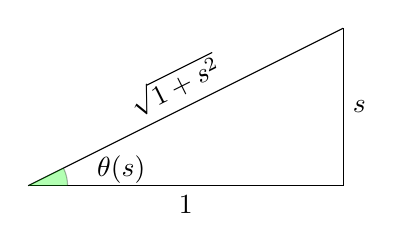
\begin{tikzpicture}
\coordinate (A) at (0,0);
\coordinate (B) at (4,0);
\coordinate (C) at (4,2);

\draw[-] (A) -- node[above,sloped] {$\sqrt{1+s^2}$} (C);
\draw[-] (A) -- node[below,sloped] {$1$} (B);
\draw[-] (C) -- node[right] {$s$} (B);

\begin{scope}
\path[clip] (A) -- node[below,sloped] {$1$} (B) -- node[right] {$s$} (C) -- node[above,sloped] {$\sqrt{1+s^2}$} (A);
\fill[green, opacity=0.3, draw=black] (A) circle (5mm);
\node at ($(A)+(10:12mm)$) {$\theta(s)$};
\end{scope}
\end{tikzpicture}
\end{wrapfigure}

\begin{gather*}
\cos θ(s) = \frac{1}{\sqrt{1+s^2}} \\
\sin θ(s) = \frac{s}{\sqrt{1+s^2}}
\end{gather*}

Integrando, tenemos que 

\begin{align*}
x(s) &= \log \left(s + \sqrt{s^2+1}\right) \\
y(s) &= \sqrt{1+s^2}
\end{align*}

Añadiendo el movimiento rígido tendríamos todas las curvas que cumplen esa ecuación:

\[ β(s) = \begin{pmatrix}
\cos θ_0 & - \sin θ_0 \\
\sin θ_0 & \cos θ_0
\end{pmatrix}\begin{pmatrix}
 \log \left(s + \sqrt{s^2+1}\right) \\
 \sqrt{1+s^2}
\end{pmatrix} + \begin{pmatrix}
x_0 \\ y_0 
\end{pmatrix} \]
\end{problem}

\begin{problem}[8] Sea $\appl{α}{I}{ℝ^2}$ PPA. Demuestra

\ppart α es segmento de recta si y sólo si $∃p_0∈ℝ^2$ por el cual pasan todas las rectas tangentes.

\ppart α es un arco de circunferencia si y sólo si $∃p_0∈ℝ^2$ que esté en todas las rectas normales.

\solution

\spart Empezamos demostrando la implicación a la derecha. Si $α$ es un segmento de recta, lo podemos escribir como 

\[ α(s) = p_0 + s\vv \]

con $\vv$ unitario. La recta tangente a $α$ en $s=s_0$ será 

 \[ α(s_0) + λα'(s_0) = p_0 + s_0\vv + λ\vv = p_0 + (s_0 + λ)\vv \]
 
y por lo tanto $p_0$ está en todas las rectas tangentes a $α$.

Ahora la implicación a la izquierda. Para $s∈I$, sabemos que la recta tangente a $α$ por $s$ es

\begin{equation}\label{eqH2E8} α(s) + λα'(s)\quad λ∈ℝ \end{equation}

Como $p_0$ está en esa recta, $∃λ(s)\tq p_0 = α(s) + λ(s)α'(s)$. Ahora la idea que se nos viene a la cabeza es derivar, pero no sabemos si λ es derivable. Despejamos y 

\[ p_0 - α(s) = λ(s)α'(s) \]

Ahora no podemos dividir por $α'$ (es un vector) así que mltiplicamos a ambos lados por $α'$:

\[ \pesc{p_α - α(s), α'(s)} =λ(s) \pesc{α'(s), α'(s)} = λ(s) \]

por lo tanto $λ(s)$ es suave en $s$. Podemos derivar, así que derivamos en (\ref{eqH2E8})

\begin{gather*}
 0 = α'(s) + λ'(s) α'(s) + λ(s) k_α(s) \mv{n}_α(s) \\
 0 = \mv{t}_α(s) + λ'(s) \mv{t}_α(s) + λ(s)k_α(s)\mv{n}_α(s) \\
 0 = (1+λ'(s))\mv{t}_α(s) + λ(s)k_α(s)\mv{n}_α(s)
 \end{gather*}
 
Dado que $\{\mv{t}_α,\mv{n}_α\}$ es una base ortonormal del plano, una combinación lineal de ambos dos sólo puede ser cero si los dos coeficientes son cero. Esto nos lleva a las dos siguientes ecuaciones

\[ \left.\begin{matrix}
1+λ'(s) = 0 \\
λ(s)k_α(s) = 0 \\
\end{matrix}\right\} ∀s∈I \]

Como $λ'(s) = -1$, $λ(s) = s_0 - s$ para algún $s_0$. Sustituimos en la segunda ecuación y nos queda que $(s_0-s)k_α(s) = 0$, así que si $s≠s_0$ $k_α(s)=0$. Y como además, $k_α$ es continua, en ese punto $s_0$ también es cero. La curvatura es cero en todo punto $s$, y por lo tanto es un segmento de recta.

\spart Visualmente, vemos que $p_0$ deberá ser el centro. La implicación a la derecha se demuestra fácilmente. Sabemos la parametrización de $α$

\[ α(s) = p_0 + r\left(\cos \frac{s}{r}, \sin \frac{s}{r}\right) \]

Calculamos la recta normal por $α(s)$ y veo que $p_0$ está en ella.

Calculamos ahora la \textbf{implicación a la izquierda}. Queremos demostrar que la curvatura es constante y distinto de 0. Sabemos que 

\[ p_0 = α(s) + λ(s)\mv{n}_α(s) \]

para algún $λ(s)$. Como podemos expresar $λ(s) = \pesc{p_0-α(s),\mv{n}_α(s)}$, es derivable. Así que derivamos.

\begin{gather*}
0 = \mv{t}_α(s) + λ'(s)\mv{n}_α(s) + λ(s)\left(-k_α(s) \mv{t}_α(s)\right) \\
0 = (1-k(s)λ(s))\mv{t}_α(s) + λ'(s)\mv{n}_α(s) 
\end{gather*}

Al igual que veíamos en el anterior apartado, sabiendo que tenemos una base normal sacamos dos ecuaciones:

\begin{gather*}
1-k(s)λ(s) = 0 \\
λ'(s)=0 
\end{gather*}

λ es constante, así que $λ(s) = c_0$ para algún $c_0∈ℝ$. Entonces

\[ 1-k_α(s)c_0 = 0 \implies k_α(s) = \frac{1}{c_0} \]

La curvatura escalar es constante, así que efectivamente trabajamos en un arco de circunferencia.

\end{problem}

\begin{problem}[9] Sea $\appl{α}{I}{ℝ^2}$ PPA. Demuestra que todas las rectas normales equidistan de un $p_0$ dado si y sólo si existen $a,b∈ℝ$ tal que \[ k_α(s) = \pm \frac{1}{\sqrt{as + b}} \]

\solution

Hagamos un dibujito

\begin{figure}[hbtp]
\centering
\begin{tikzpicture}[pnt/.style={draw,shape=circle,fill=white, inner sep=2pt}]
\draw[-] (0,0) -- (6,0);
\node[pnt,label=below:{$α(s)$}] (S) at (2,0) {};
\node[label=below:{$\cn(s)$}] (N) at (3.5,0) {};
\node[pnt] (PA) at (4,0) {};
\draw[thick,->] (S) -- (N);
\draw[->] (S) -- node[left] {$-\mv{t}_α(s)$} (2,2);
\node[pnt,label=right:{$p_0$}] (P) at (4,3) {};
\draw[->] (S) -- node[midway, above, sloped] {$p_0-α(s)$} (P);
\draw[dashed] (P) -- node[right] {$\pesc{p_0-α(s), -\mv{t}_α(s)}$} (PA);
\end{tikzpicture}
\end{figure}

Derivamos la distancia $\pesc{p_0-α(s), -\mv{t}_α(s)}$

\[ 0 = \pesc{-\mv{t}_α(s),-\mv{t}_α(s)} + \pesc{p_0-α(s),-k_α(s) \mv{n}_α(s)} \]

y por lo tanto $k_α(s)\pesc{p_60-α(s),\mv{n}_α(s)} = 1$. Volvemos a derivar (total, es gratis)

\[ \cv(s)\pesc{p_0-α(s)\cn(s)} + \cv(s)\left(\pesc{\ct(s), \cn(s)} + \pesc{p_0-α(s), -\cv(s)\ct(s)}\right) = 0 \]

y dividimos:

\[ \frac{\cv'(s)}{\cv(s)} - c\cv^2(s) = 0 \]

Resolvemos la ecuación diferencial y nos queda que

\[ \frac{-1}{2k^2}=cs + d \]

Por lo tanto

\[ k^2 = \frac{1}{(-2c)s + (-2d)} \]

de tal forma que hemos llegado a la fórmula que nos daban al principio.

Ahora vamos a por la \textbf{otra implicación}. Pero no, que es muy larga.
\end{problem}

\begin{problem}[11] Sea $Γ$ una curva cerrada, simple, en el plano, contenida en el interior de la circunferencia $\{ x^2+y^2=r^2 \}$. Demuestra que existe un punto $p∈Γ$ tal que $\md{k(p)} ≥ \frac{1}{r}$.

\solution

Partimos de que $\frac{1}{r}$ es la curvatura del círculo. Trasladamos la circunferencia en cualquier dirección hasta tocar la curva por primera vez. En ese punto de contacto, la tangente es la misma y por lo tanto la normal también.

Si trasladásemos y rotamos las curvas para que el plano sea el eje $OX$ y el punto de contacto fuese el origen, tendríamos algo parecido a la imagen \ref{imgCirc}.

\easyimg{img/Hoja2_11_CircCurva.png}{Curva y circunferencia}{imgCirc}

Si podemos escribir la curva $α=α(s)$ como grafo de una función $h_1(x)$, entonces

\[ k(α(0)) = \frac{h_1''(x)}{\left(1+h_1'(x)^2\right)^{\frac{3}{2}}} \]

Dado que tenemos un grafo sobre la recta tangente, $h_1'(0) = 0$ y entonces $k_Γ(0)=h_1''(0)$. Por otra parte, sabemos que $k_C(0) = h_2''(0) = \frac{1}{4}$. Además, $h_1(x) ≥ h_2(x)$ en un intervalo $(-δ,δ)$ y las funciones y sus derivadas valen lo mismo en $0$. Por lo tanto, tiene que cumplirse

\[ h_1''(0) ≥ h_2''(0) \implies k_Γ(0) ≥ \frac{1}{r} \]

\end{problem}


\subsection{Hoja 3}

\begin{problem}[2] Tenemos una curva $α=α(s)$ PPA biregular. Demuestra que 

\[ \ctr (s) = \frac{α'(s) × α''(s) \cdot α'''(s)}{\abs{\cv(s)}^2} \]

\solution

Sabemos que 

\begin{align*}
α'(s) &= \ct (s) \\
α''(s) &= \ct'(s) = \cv (s) \cn (s) \\
α'''(s) &= \cv'(s) \cn(s) + \cv(s) \cn'(s) = \\
&= \cv'(s) \cn(s) + \cv(s) \left(-\cv(s)\ct(s) + \ctr(s) \cb(s) \right)
\end{align*}

Mientras arreglaba una cosa de \LaTeX me ha escrito una pizarra y me he perdido. Así que nada.

\end{problem}

\begin{problem}[3] Sea $α(s)$ una curva birregular PPA, con $\cv$ y $\ctr$ curvatura y torsión. Dado $β(s) = \ct(s)$, comprobar que es regular y que 

\[ \cvv[β] = \frac{\ctr}{\cv}\cb(s) - \ct(s) \]

\solution

\spart Defino $β(s) = \ct(s)$. Comprobamos si es regular

\[ β'(s) = \ct'(s) = \cv(s) \cn (s) ≠ 0 \]

ya que $k_α(s)≠0$ para todo $s$ ya que α es birregular.

\spart Queremos demostrar que

\[ \cvv[β] = \frac{\ctr}{\cv}\cb(s) - \ct(s) \]

No sabemos si β está parametrizada por arco. Viendo la ecuación anterior, $\md{β'} = \md{\cv}$, que es distinto de uno si la curvatura no es constante igual a 1 y por lo tanto β no es PPA.

En esta situación tenmos varias posibilidades. O bien primero reparametrizamos β por arco $r$ tal que $β(s(r)) = γ(r)$ y hallo $γ''(r)$ o bien hallo $\cvv[β](s)$  usando la fórmula para curvas no PPA. 

\paragraph{Reparametrización por arco} Sea $r$ el parámetro de arco de β. Entonces

\[ r(s) = \int_{s_0}^s \md{β'(z)}\dif z = \int_{s_0}^s \cv(z) \dif z;\quad r'(s) = \cv(s) \] 

Sea $γ(r) = β(s(r))$ la reparametrización de β por arco $r$. Hallamos las dos derivadas de γ:

\[ γ'(r) = β'(s(r)) · s'(r) = \cv(s(r)) \cn(s(r)) · \frac{1}{\cv(s(r))} = \cn (s(r)) \]

\begin{align*} 
\cv[γ](r) &= γ''(r) = \cn'(s(r)) s'(r) =& \text{(Eqs. Frenet)}\\
  &= \left (-\cv(s(r))\ct(s(r)) + \ctr(s(r))\cb(s(r))\right) \frac{1}{\cv(s(r))} =& \\
  &= \frac{\ctr}{\cv}\cb(s) - \ct(s) &
\end{align*}

\end{problem}

\begin{problem}[4]
Sea $\appl{α}{I}{ℝ^3}$ curva birregular y PPA. Todas sus rectas normales pasan por el mismo punto $p_0$. Demuestre que la traza de α está contenida en una circunferencia.

\solution

Sabemos que una circunferencia dentro de un plano tiene curvatura constante y torsión 0, con el recíproco también cierto. Vamos a demostrar que si todas las rectas normales pasan por el mismo punto, tienen que darse esas dos condiciones sobre la curvatura y torsión.

Escribimos la condición de las rectas normales. Para un punto $s$ en la curva, la recta normal es

\[ α(s) + λ(s)\cn(s) = p_0 \]

con $λ(s)∈ℝ$. Derivamos:

\begin{gather*}
\ct + λ'\cn + λ\cn' = 0 \\
\ct + λ'\cn + λ(-\cv \ct + \ctr \cb) = 0
\end{gather*}

Dado que $\ct$, $\cb$ y $\cn$ forman una base l.i. del diedro ortonormal, para que esa ecuación sea 0 todos los coeficientes han de ser 0. Es decir

\[ 1-\cv λ = 0;\quad λ' = 0;\quad λ\ctr = 0 \]

De $λ'=0$ obtenemos que $λ=c_0≠0$, por lo que 

\begin{align*}
1-\cv λ = 0 &\implies \cv = \frac{1}{c_0} \\
λ\ctr = 0 &\implies \ctr = 0
\end{align*}

Ambos resultados implican que α es un trozo de circunferencia.
\end{problem}

\begin{problem}[7] Sea $\appl{α}{I}{ℝ^3}$ PPA con $\cv > 0$. Demostrar que $α(I)$ es un arco de circunferencia si y sólo si $\cv$ es constante y α está contenida en una esfera.

\solution

La implicación a la derecha es trivial. Muy trivial. 

Para la implicación a la izquierda, tenemos que ver que $\ctr\equiv 0$, ya que por hipótesis nos han dicho que $\cv$ es constante. Dado que α está contenida en la esfera, la condición la escribimos como

\[ \md{α(s) - p_0}^2 = R^2 \]

para $p_0$ el centro de la esfera. Dado que eso es una función de una variable y tiene que ser constante, derivamos porque a este hombre le encanta derivar

\[ f'(s) = 2\pesc{\ct,α(s)-p_0} = 0 \]

\begin{center}\Huge{Más derivadas}\end{center}

\[ \frac{f''(s)}{2} = \pesc{\ct', α(s)-p_0} + \pesc{\ct, \ct} \]

Que podemos reexpresar que 

\[ \pesc{\cn, α(s) - p_0} = \frac{-1}{\cv} \]

Y...

\easyimg{img/DERIVADAS.png}{DERIVAAAAAMOOOOOOOOOOOOOS}{imgDerivadas}

\begin{gather*}
 \pesc{\cn', α(s)-p_0} + \pesc{\cn, \ct} = 0 \\
 \pesc{-\cv\ct + \ctr\cb, α(s)-p_0} = \ctr \pesc{\cb, α(s)-p_0} = 0
 \end{gather*}
 
 Suponemos que existe un $s_0$ donde $\ctr(s_0)≠0$. En un entorno alrededor de ese punto, se tiene que 
 
 \[ \pesc{\cb, α(s)-p_0} = 0 \]
 
 Entonces
 
 \begin{gather*}
  α(s)-p_0 = \frac{1}{\cv}\cn(s) \\
  α(s) = p_0 - \frac{1}{\cv}\cn(s) \\
  \ct = \frac{1}{\cv}\left(-\cv\ct + \ctr \cb\right) \\
  \frac{-\ctr}{\cv}\cb = 0
  \end{gather*}
  
  Lo que nos llevaría a que $\ctr=0$, contradicción.
 
\end{problem}


\subsection{Hoja 4}

\begin{problem}[1] Sea $f(x) = (x+y+z-1)^2$. Halle los valores y puntos críticos de $f$. Decida para qué valores $c$, $\inv{f}(c)$ es una superficie regular.

\solution

Calculamos las derivadas parciales:

\[ f_x = f_y = f_z = 2(x + y + z -1) \]

Igualando a cero, tenemos que los puntos críticos están en el plano

\[ x+ y+z = 1 \]

y el único valor crítico es el 0.

Ahora nos piden buscar para qué valores $c∈ℝ$ $\inv{f}(c)$ es una superficie regular. Consideramos varias opciones.

\begin{itemize}
\item Si $c<0$, $\inv{f}(c)= \emptyset$ y no es superficie regular.
\item Si $c>0$, $\inv{f}(c) ≠\emptyset$. Por ejemplo $P=(\sqrt{c} + 1, 0,0∈\inv{f}(c)$ y como $c$ no es valor crítico, $f^{-1}(c)$ es superficie regular.
\item Si $c=0$, antes habíamos calculado que ese era un valor crítico para los puntos críticos del plano $x+ y+z = 1$, así que efectivamente es una superficie regular.
\end{itemize}

\end{problem}

\begin{problem}[6] Sean $r,R>0$ y $r<R$. Llamamos toro $T$ al conjunto de puntos $(x,y,z)$ obtenidos al girar alrededor del eje $OZ$ la circunferencia $C$ de centro $(0,R,0)$, radio $r$ y situada en el plano $x=0$.

Demuestra que $T$ se puede expresar como un conjunto de nivel $T=\inv{F}(0)$ de una función $\appl{F}{ℝ^3}{ℝ}$, con 

\[ F(x,y,z) = (x^2+y^2+z^2-R^2-r^2)^2-4R^2(r^2-z^2) \]

\solution

Partimos del siguiente dibujo.

\easyimg{img/Hoja4_6_Toro.png}{Planteamiento del problema.}{imgToro}

Proponemos que todo punto de $T$ lo obtengo a partir de un $p_0$ en $C$ tras rotarlo un cierto ángulo θ con respecto al eje $OX$. Entonces, la parametrización es

\(\label{eqH4_6_Param} \begin{matrix}
x &=& (R + r\cos ψ)\cos θ \\
y &=& (R + r\cos ψ)\sin θ \\
z &=& r\sin ψ
\end{matrix} \)

¿Cómo demostramos que ambos conjuntos $T$ y $\inv{F}(0)$ son iguales? Pues lo de siempre: doble contención. Primero vemos si $T⊆\inv{F}(0)$.

Calculamos $F(T)$. Para $(x,y,z)∈T$, 

\[ F(x,y,z) = \dotsb =\footnote{Magia!} 0 \]

Vamos ahora al revés: queremos mirar si $\inv{F}(0)⊆T$. Si $(x,y,z)∈\inv{F}(0)$, sabemos que

\[ (x^2+y^2+z^2-R^2-r^2)^2 = 4R^2(r^2-z^2) \]

Hay que buscar $θ,ψ$ para que se cumpla \eqref{eqH4_6_Param}.

\end{problem}


\subsection{Hoja 5}

\paragraph{Primera forma fundamental} Tenemos una superficie $S$, una forma cuadrática

\begin{align*}
\appl{I_p}{T_pS&}{ℝ} \\
v \mapsto \pesc{v,v}
\end{align*}

y una parametrización $\appl{Φ}{U}{S}$ que lleva un punto $(u,v)$ a $p=Φ(u,v)$. $\{Φ_u(u,v),Φ_v(u,v)\}$ es una base del plano tangente $T_pS$. Para hallar la forma fundamental, hallamos ese producto escalar 

\[ I_p(v) = \pesc{aΦ_u + bΦ_v, aΦ_u + bΦ_v} = a^2\underbrace{\pesc{Φ_u,Φ_u}}_{E(u,v)} + 2ab \underbrace{\pesc{Φ_u, Φ_v}}_{F(u,v)} + b^2 \underbrace{\pesc{Φ_v,Φ_v}}_{G(u,v)} \]


\paragraph{Cálculo del ángulo entre curvas} Si tenemos dos curvas $\appl{α,β}{I}{S}$ que se cortan en un punto $p=α(t_0) = β(s_0)$, entonces el coseno del ángulo $θ$ de corte es

\[ \cos θ = \frac{\pesc{α'(t_0), β'(s_0)}}{\norm{α'(t_0)}\norm{β'(s_0)}} \]

Nos pueden dar la primera forma fundamental de una superficie $Φ(u,v)$ de tal forma que 

\begin{align*}
α(t) &= Φ(u_1(t), v_1(t)) \\
β(t) &= Φ(u_2(s), v_2(s))
\end{align*}

Entonces, podemos expresar las derivadas como

\begin{align*}
α'(t_0) &= u_1'(t_0) Φ_u + v_1'(t_0) Φ_v \\
β'(s_0) &= u_2'(s_0) Φ_u + v_2'(s_0) Φ_v 
\end{align*}

y nos queda

\[ \pesc{α'(t_0),β'(s_0)} = \begin{pmatrix}
u_1' & v_1'
\end{pmatrix} 
\begin{pmatrix}
E & F \\
F & G
\end{pmatrix}
\begin{pmatrix}
u_2' \\ v_2 '
\end{pmatrix} \]

Sólo faltaría hallar las normas, que se haría como  \[ \norm{α'(t_0)}^2 = E(u_1')^2 + 2Fu_1'v_1' + G(v_1')^2 \].

En particular, podemos hallar el ángulo entre las curvas coordenadas $α=Φ(t,v_0)$ y $β=Φ(u_0, s)$. En este caso, 
\begin{align*}
α' &= Φ_u \\
β' &= Φ_v 
\end{align*}

y en el numerador nos queda $Φ_uΦ_v = F$. Es decir, que

\[ \cos θ = \frac{F}{\sqrt{EG}} \]

\begin{problem}[2] Hallar la primera forma fundamental de una superficie con parametrización 

\[ Φ(u,v) = (au\cosh v, bu\sinh v, u^2) \]

\solution Para hallar los coeficientes, derivamos:

\begin{align*}
Φ_u &= (a\cosh v, b\cosh v, 2u) \\
Φ_v &= (au\sinh v, bu\sinh v, 0)
\end{align*}

Ahora tenemos que hallar los coeficientes de la primera forma fundamental haciendo los productos escalares:

\begin{align*}
E(u,v) &= \pesc{Φ_u,Φ_u} &= a^2\cosh^2v + b^2\sinh^2v + 4u^2 \\
F(u,v) &= \pesc{Φ_u,Φ_v} &= (a^2+b^2)u\sinh v \cosh v \\
G(u,v) &= \pesc{Φ_v,Φ_v} &= a^2u^2\sinh^2 v + b^2u^2\cosh^2v 
\end{align*}

\end{problem}

\paragraph{Cálculo del área a través de la primera forma fundamental} Supongamos que queremos calcular el área de una región $R=φ(U)$. Normalmente, escribiríamos

\[ \mop{\'Area}(R) = \iint_U \norm{Φ_u× Φ_v}\id{u,v} \]

Con los coeficientes de la primera forma fundamental, esto coincide con

\[ \mop{\'Area}(R) = \iint_U \sqrt{EG - F^2} \id{u,v} \]

\begin{problem}[3] Hallar el área de la superficie de revolución dada por el giro de la curva PPA

\[ α(t) = (0, ρ(t), h(t)) \]

\solution La parametrización de la superficie de revolución con respecto al eje $Z$ será

\[ Φ(u,v) = (ρ(v)\cos u, ρ(v) \sin u, h(v)) \]

Hallamos la primera forma fundamental, primero derivando

\begin{align*}
Φ_u &= (-ρ(v)\sin u, ρ(v) \cos u, 0 ) \\
Φ_v &= (ρ'(v)\cos u, ρ'(v) \sin u, h'(v))\\
\end{align*}

lo que nos da los coeficientes

\begin{align*}
E = ρ^2(v) \\
F = 0 \\
G = ρ'^2 + h'^2 = \norm{α'}^2 \stackrel{PPA}{=} 1
\end{align*}

Vemos que salen valores \textit{curiosos}. Estudiamos $F$, que era $ \pesc{Φ_u,Φ_v}$. Como vale 0, esto indica que los vectores $Φ_u$ y $Φ_v$ son ortogonales, algo que parece muy lógico si vemos que $Φ_u$ es siempre tangente a la circunferencia de revolución, y $Φ_v$ es tangente a la curva.

Hallamos ahora el área:

\[ \mop{\'Area}(S) = \int_a^b \int_0^{2π} \sqrt{ρ^2(v)} \id{u,v} = 2π \int_a^b ρ(v) \dif v \]


\end{problem}

\begin{problem}[5] Tenemos la siguiente parametrización de una superficie $S$

\[ Φ(u,v) = (u\cos v,u \sin v, \log \cos v + u) \]

con $u∈ℝ$, $v∈\left(\frac{-π}{2}, \frac{π}{2}\right)$. Demostrar que el par de curvas $Φ(u_1,v)$, $Φ(u_2,v)$ cortan a cada curva $Φ(u,v_0)$ con igual longitud.

\solution Supongamos que $v$ es el parámetro \textit{vertical} y $u$ el \textit{horizontal}.

\begin{figure}[htbp]
\centering
\begin{tikzpicture}[scale=3]
\coordinate (A) at (0,0) {};
\coordinate (B) at (1,0) {};
\coordinate (C) at (1,1) {};
\coordinate (D) at (0,1) {};

\draw[-] (-0.1,-0.3) edge[out=90,in=270] (A) (A) -- (D) to[out=90,in=270, looseness=1]  (0.1,1.3) (0.1,1.3)  node[above] {$Φ(u_1, v)$};
\draw[-] (0.9,-0.3) edge[out=90,in=270] (B) (B) -- (C) edge[out=90,in=270]  (1.1,1.3) (1.1,1.3)  node[above] {$Φ(u_2, v)$};
\draw[-] (-0.3,0.4) edge[out=0,in=180] (0,0.5) (0,0.5)-- (1,0.5) edge[out=0,in=180]  (1.3,0.6) (1.3,0.6) node[right] {$Φ(u, v_0)$};

\draw[-,green!20!black,very thick] (0,0.5) -- node[midway,below] {$α_{v_0}$} (1,0.5);

\end{tikzpicture}
\end{figure}

Llamamos $α_{v_0} = Φ(t,v_0)$, con $t∈[u_1, u_2]$ a la curva desde la primera a la segunda curva. Su longitud será entonces

\[ L(α_{v_0}) = \int_{u_1}^{u_2} \norm{α_{v_0}'(t)} \dif t \]

Uno diría que ya ha terminado, pero falta calcular el vector tangente. Pero ese es el camino desesperado, nosotros somos listos y vemos que el vector del que hallamos la norma es $Φ_u(t,v_0)$. Entonces

\[ \norm{α_{v_0}'(t)} \pesc{Φ_u(t,v_0), Φ_u(t,v_0)}^{\frac{1}{2}} = E(t,v_0)^{\frac{1}{2}} \]

No hemos simplificado mucho, pero bueno, integramos y a ver qué pasa.

\[ Φ_u(t,v_0) = (\cos v_0, \sin v_0, 1) \implies E = 2 \]

y por lo tanto

\[ L(α_{v_0}) = \int_{u_1}^{u_2} \sqrt{2} \dif t = \sqrt{2} (u_2 - u_1) \]

No hemos ganado mucho, así que vamos a hacer otra curva.
\end{problem}

\begin{problem}[9] En una parametrización $Φ(u,v)$, la 1FF es 

\[ Q = \dif u^2 + 2(u+v) \id{u,v} + e^v \dif v^2 \]

Introduzco nuevas coordenadas $(λ,μ)$ tales que

\begin{align*}
u &= e^λ + μ \\
v &= μ
\end{align*}

Halla $\tilde{Q}$, la 1FF en las coordenadas $(λ,μ)$.

\solution Tenemos dos formas para solucionar. Derivamos

\begin{gather*}
u = e^λ + μ \\
\dif u = e^λ \dif λ + \dif μ \\
\dif v = \dif μ
\end{gather*}

Entonces

\begin{align*}
\dif u^2 &= e^{2λ} \dif λ^2 + 2e^λ \dif λ \dif μ + \dif μ^2 \\
\dif u \dif v &= e^λ \dif λ \dif μ + \dif μ^2 \\
\dif v^2 &= \dif μ^2
\end{align*}

Si $Q = \dif u^2 + 2(u+v) \id{u,v} + e^v \dif v^2$, sustituimos

\[  \tilde{Q} = e^{2λ} \dif λ^2 + 2e^λ \dif λ \dif μ + \dif μ^2 + 2 + \\ (2e^λ + 2μ)(e^λ \dif λ \dif μ + \dif μ^2) + e^μ \dif μ^2
\]
Agrupamos coeficientes:

\[ \tilde{Q} = \underbrace{e^{2λ}}_{\tilde{E}} \dif λ^2 + \underbrace{(2e^λ + (2e^λ + 2μ)e^λ)}_{\tilde{F}}\dif λ \dif μ + \underbrace{(1+ (2e^λ + 2μ) + e^μ)}_{\tilde{G}} \dif μ^2 \]

\paragraph{Segunda forma}

Tenemos $Φ(u,v)$ que nos da los coeficinetes $E, F, G$. Con el cambio de variables al que llamamos $T$ podemos construir $ψ(λ,μ) = Φ ○ T$. Entonces, por ejemplo, $\tilde{E} = \pesc{ψ_λ,ψ_λ}$. Pero

\[ ψ_λ = Φ_ue^λ + Φ_v · 0 = e^λ Φ_u \]

así que sustituimos:

\[ \tilde{E}(λ,μ) = \pesc{e^{2λ}Φ_u, e^{2λ}Φ_u} = e^{2λ}E(e^λ + μ, μ) = e^2λ \]

Etc\ae tera, etc\ae tera.

\end{problem}

\paragraph{Cálculo de isometrías} Tenemos un abierto $U⊆ℝ^2$, con parámetros $(u,v)$, y dos parametrizaciones sobreyectivas

\begin{align*}
\appl{Φ&}{U}{S} \\
\appl{ψ&}{U}{S'}
\end{align*}

Tenemos también una aplicación $\appl{h}{S}{S'}$ tal que $h(Φ(u,v)) = ψ(u,v)$.

Entonces $h$ es isometría si y sólo si la primera forma fundamental de $S$ en la parametrización $φ$ es la misma que la 1ff de $S'$ en la parametrización $Ψ$. Es decir

\begin{align*}
E_Φ (u,v) &= E_ψ(u,v) \\
F_Φ (u,v) &= F_ψ(u,v) \\
G_Φ (u,v) &= G_ψ(u,v) 
\end{align*}.

El esquema de lo que ocurre está en la figura \ref{imgH5E1}. Es un diagrama conmutativo.

\begin{figure}[hbtp]
\centering
\begin{tikzpicture}[x=2cm,y=2cm]
\node (S) at (0,1) {$Φ(u,v) ∈ S$};
\node (S2) at (2,1) {$ψ(u,v) ∈ S'$};
\node (U) at (1,0) {$(u,v) ∈ U$};

\draw[->] (S) -- node[above] {$h$} (S2);
\draw[->] (U) -- (S);
\draw[->] (U) -- (S2);
\end{tikzpicture}
\label{imgH5E1}
\caption{Diagrama de las aplicaciones definidas.}
\end{figure}

Podemos ver que si $\appl{Φ}{U}{S}$ es inyectiva, tengo una inversa $\appl{\inv{Φ}}{S}{U}$ y entonces podríamos reescribir $h$ como $h = ψ ○ \inv{Φ}$.

\begin{problem}[1] Consideramos dos parametrizaxiones

\begin{align*}
\appl{Φ&}{ℝ^2}{S} \\
\appl{ψ&}{ℝ^2}{S'}
\end{align*}
con
\begin{align*}
Φ(u,v) &= \left(u^3+3u, \frac{3}{5}, \frac{3}{5}v^5 - 3v, 4u^2 + \frac{10}{3}v^3 \right)\\
\end{align*}

Demuestra que $\appl{h}{S}{S'}$ con $h(Φ(u,v)) = ψ(u,v)$ existe y es una isometría.

\solution

Tenemos que demostrar que existe la inversa de Φ, así que como $S=Φ(ℝ^2)$ sólo tenemos que demostrar la inyectividad. Buscamos resolver $Φ(u,v) = Φ(\bar{u},\bar{v})$:

\begin{align*}
u^3+3u &= \bar{u}^3 + 3\bar{u} \\
\frac{3}{5}v^5 - 3v &= \frac{3}{5}\bar{v}^5 - 3\bar{v} \\
4u^2 + \frac{10}{3}v^3 &= 4\bar{u}^2 + \frac{10}{3}\bar{v}^3
\end{align*}

¿Cómo lo hacemos? En lugar de resolver el sistema, vemos que en la primera ecuación, la primera derivada es $3u^2 + 3$, que es siempre positivo. Por lo tanto, la primera coordenada es siempre creciente e inyectiva y entonces $u=\bar{u}$. Sustituyendo en la última ecuación, eliminamos la $u$ y nos queda que $\bar{v} = v$.

Para que $h$ sea isometría tiene que ser un difeomorfismo y que preserve la primera forma fundamental. Por lo tanto, necesitamos ver que $ψ$ es biyectiva, que lo es porque sí.

Si hacemos los cálculos de los coeficientes de la 1ff para Φ y ψ, vemos que son iguales y por lo tanto es una isometría.
\end{problem}


\subsection{Hoja 6}

\begin{problem}[1] Consideramos una superficie $C⊆ℝ^3$ que es un \textit{"cono"}, generado trazando rectas desde un punto fijo (vértice) hasta todos los puntos de una curva cualquiera (no tiene por qué ser una circunferencia.

Sea $S_1$ la esfera unidad centrada en el origen, y α la intersección del cono con $S_1$. $α(u)$ es una parametrización, y entonces tomamos $Φ(u,v) = vα(u)$ con $v>0$.

Comprueba que si $α$ es PPA, la 1FF de $Φ$ es la misma para cualquier cono.

\solution

Calculamos la 1FF:

\[ \begin{cases}
Φ_u = vα'(u) \\
Φ_v = α(u) \\
\end{cases}\implies \begin{cases}
E &= v^2α'^2(u) = v^2 \\
F &= vα'(u)α(u) = 0\\
G &= α^2(u) = 1
\end{cases} \]

Es decir, la curva no influye en ningún momento y por lo tanto la 1FF de $Φ$ es siempre la misma.
\end{problem}

\begin{problem}[3] Sea $Σ$ parametrizada por 

\[ Φ(u,v) = \left(r(u)\cos v,r(u)\sin v,z(u)\right) \].

Además, la normal unitaria es

\[ N = \left(-z'(u) \cos v, -z'(v) \sin v, r'(u) \right) \]

Calcular la primera y segunda forma fundamental, y algo sobre las curvaturas principales.
\solution

Podemos ver que $Σ$ es una superficie de revolución de la curva $(r(u), 0, z(u))$. Además, viendo la normal unitaria tenemos que $z'^2 + r'^2 = 1$, y por lo tanto la curva de revolución está parametrizada por arco. 

Calculamos la 1ff y la 2ff:

\begin{align*}
Φ_u &= \left(r' \cos v, r'\sin v, z'\right) \\
Φ_v &= \left(-r\sin v, r\cos v, 0\right) \\
Φ_{uu} &= \left(r''\cos v, r''\sin v, z''\right) \\
Φ_{uv} &= \left(-r' \sin v,-r'\cos v, 0\right) \\
Φ_{vv} &= \left(-r\cos v, -r \sin v, 0\right)
\end{align*}
lo que nos da los coeficientes
\begin{align*}
E &= r'^2 + z'^2 = 1 \\
F &= 0 \\
G &= r^2 \\
e &= \pesc{N,Φ_{uu}} = -r''z' + r'z''\\
f &= \pesc{N,Φ_{uv}} = rz'\\
g &= \pesc{N,Φ_{vv}} = rz' \\
\end{align*}

Pero además, al haber calculado antes la primera forma fundamental, podríamos sacar que

\[ N = \frac{Φ_u × Φ_v}{\norm{Φ_u×Φ_v}} = \frac{Φ_u × Φ_v}{\sqrt{EG-F^2}} 
\] y que además

\[ e = \pesc{N,Φ_{uu}} = \frac{1}{\sqrt{EG-F^2}} \det [ Φ_u | Φ_v | Φ_{uu} ] \]

De esta forma evitamos realizar cuentas excesivamente complejas.

Siguiendo con el ejercicio, la segunda forma fundamental sería

\[ Π_Φ = (-r''z'+r'z'')\dif u^2 + 2·0·\dif u \dif v + rz'\dif v ^2 \]

Hallemos ahora las \textbf{curvaturas principales}. La primera aplicación es $\appl{?}{T_pS}{T_pS}$ que lleva un vector $v$ a un vector $\Dif_vN$. La matriz de la aplicación está dada por 

\[ \begin{pmatrix}
E & F \\ F & G
\end{pmatrix}^{-1}
\begin{pmatrix}
e & f \\ f & g
\end{pmatrix} = \begin{pmatrix}
-r''z' + r'z'' & 0 \\ 0 & \frac{z'}{r}
\end{pmatrix}\]

Las curvaturas principales son los autovalores de esa matriz, que como es diagonal ya los tenemos escritos.

Si por ejemplo nos hubieran dado la curvatura gaussiana $K$ y la media $H$, podríamos recuperar las curvaturas principales $k_1,k_2$ a través de sus respectivas fórmulas:

\begin{gather*}
 K = k_1k_2 \\
 H = \frac{-(k_1 + k_2)}{2}
\end{gather*}

\end{problem}

Una curva α es asintótica cuando $II_{α(t)}(α'(t)) = 0$. Es decir, la curva siempre va buscando ser tangente a una dirección que anule la 2FF.

\begin{problem}[6] \textbf{Limones localmente isométricos a la esfera.} Tenemos la esfera sin un meridiano dada por la parametrización
\[
Φ(u,v) = (\cos u\cos v,\cos u \sin v, \sin u)\quad u∈\left(-\frac{π}{2},\frac{π}{2}\right),\;v∈(0,2π) 
\]
que es una superficie de revolución de la semicircunferencia dada por $ρ(u) = \cos u$, $h(u) = \sin u$.

\ppart Para cada $c>1$ encuentra $r_c(u), z_c(u)$ con $u∈\left(-\frac{π}{2},\frac{π}{2}\right)$ tal que si \[ ψ^c(u,μ) = \left(r_c(u)\cos μ, r_c(u)\sin μ, z_c(u)\right) \] con $μ∈ℝ$, entonces la aplicación $\appl{h}{S}{S_c}$ que a $Φ(u,v)$ le asigna $ψ^c(u,cv)$ es isometría local.

\solution

Para que $h$ sea isometría, la 1FF de Φ y ψ tienen que ser iguales. Nos molesta la $c$ que están en $ψ(u,cv)$ para poder aplicar lo que veíamos en el problema 1 de la hoja 5, así que vamos a arreglar esto.

Sea $ Γ(u,v) = ψ^c(u,cv)$. Basta ver que los coeficientes de la primera forma fundamental de Φ y de Γ coinciden. Vamos a calcularlos:

\begin{align*}
E_Φ &= 1\\
F_Φ &= 0\quad \text{(sup. de revolución)} \\
G_Φ &= \cos^2 u \\
\end{align*}

Calculamos las derivadas de Γ
\begin{gather*}
Γ_u = (r_c' \cos cv,r_c'\sin cv,z_c') \\
Γ_v = (-r_c'c\sin cv, r_c c \cos cv, 0) 
\end{gather*}
y obtenemos los coeficientes

\begin{align*}
E_Γ &= r_c'^2 + z_c'^2 \\
F_Γ &= 0 \\
G_Γ &= c^2r^2
\end{align*}.

Igualamos los coeficientes y tenemos

\begin{align*}
r_c'^2 + z_c'^2 &= 1 \\
c^2r^2(u) &= \cos^2 u
\end{align*} lo que nos da las dos funciones

\begin{gather*}
z_c(u) = \int\sqrt{1-\frac{1}{c^2}\sin^2u}\dif u \\
r_c(u) = \frac{1}{c}\cos u
\end{gather*} 

El enunciado ahora nos pide ver qué le ocurre al ecuador de esta superficie cuando $c$ aumenta, y lo que vemos es que se acerca al eje del origen.

También nos pide demostrar que la altura del limón es creciente en $c$. La altura del limón es

\[ z_c\left(\frac{π}{2}\right)-z_c\left(\frac{-π}{2}\right) = \int_{-π/2}^{π/2} \sqrt{1-\frac{1}{c^2} \sin^2 s}\dif s = f(c) \]. 

Obtenemos la derivada

\[ f'(c) = \int_{-π/2}^{π/2} \left(1-\frac{1}{c^2}\sin s\right)^{\frac{-1}{2}} · \frac{1}{2} · \frac{2}{c^3} \sin^2 s \dif s 
\]
que es siempre positiva, y por lo tanto es creciente. Cuando $c\to ∞$, converge a \[\lim_{c\to ∞} \int_{-π/2}^{π/2} \sqrt{1-\frac{1}{c^2}\sin^2u}\dif u = \int_{-π/2}^{π/2} 1 = π \].

Vamos ahora con las \textbf{curvaturas principales}. En el ejercicio anterior se dice que una superficie de revolución $(r(u),z(u))$ tiene curvaturas principales \[ r'z'' - r''z',\quad \frac{z'}{r} \]. Queremos saber si conserva la isometría $h_c$ el par no ordenado de curvaturas principales. En nuestro caso, derivando y operando

\begin{gather*}
 r'z'' - z'r'' = \frac{1}{c}\cos u \left(1-\frac{1}{c^2}\sin^2 u\right)^{-\frac{1}{2}} \\
 \frac{z'}{r} = \frac{\left(1-\frac{1}{c}\sin^2 u\right)^{1/2}}{\frac{1}{c}\cos u}
 \end{gather*}

¿Para qué queremos todos estos cálculos? Los limones son localmente isométricos a la esfera. La esfera tiene curvaturas principales iguales a $1$ en todos los puntos. Sin embargo, nuestros limones tienen curvaturas principales distintas. De aquí podemos extraer la sabia lección de que una isometría local no conserva las curvaturas principales.

Pero hay otra cosa: el producto de las curvaturas principales es igual a la curvatura gaussiana. La curvatura gaussiana de la esfera es uno, y la de los limones es también uno. Es decir, \textbf{la curvatura gaussiana} se conserva en las isometrías locales.
\end{problem}

\begin{problem}[7] Sea $α(u)$ una curva birregular en el espacio PPA. Sea $S$ la parte de la superficie tangencial dada por la parametrización \[ Φ(u,v) = α(u) + v \ct(u) \] con $v > 0$.

Describe la normal unitaria $N(u,v)$ de $S$ en términos del triedro de Frenet $\{\ct(u), \cn(u),\cb(u)\}$ de α. A partir de eso, calcula el endomorfismo de Weingarten de $S$ sin pasar por la segunda forma fundamental. Demuestra que cada punto de $S$ es parabólico o plano. ¿Cuándo tiene $S$ puntos planos?

\solution

Calculamos las derivadas

\begin{align*}
Φ_u &= \ct(u) + v \cv(u) \cn(u) \\
Φ_v &= \ct(u)
\end{align*}, el producto vectorial

\[ 
Φ_u×Φ_v = 0 + v\cv(u) (-\cb(u)) 
\]
y por último la normal unitaria
\[
N = \frac{Φ_u×Φ_v}{\norm{Φ_u×Φ_v}} = \frac{-v\cv(u)\cb(u)}{\norm{-v\cv(u)\cb(u)}} = - \cb(u) \].

Vamos a calcular ahora el \textbf{endomorfismo de Weingarten} sin usar la 2FF. ¿Cómo calculamos esta cosa? Tenemos que calcular la aplicación $\appl{\dif N}{T_pS}{T_pS}$ evaluada en $Φ_u$ y en $Φ_v$. Es

\begin{gather*}
 \dif N (Φ_u )= \od{}{s}(N(u+s,v)) = N_u = \od{}{u} ( -\cb(u)) = -\cb'(u) = \ctr(u) \cn (u) \\
 \dif N (Φ_v) = N_v = \od{}{s}(-\cb(u)) = 0
 \end{gather*}

Tenemos que escribir $\dif N(Φ_u)$ en función de $Φ_u$ y $Φ_v$, entonces

\[ \ctr \cn = a Φ_u + b Φ_v =  a \ct + a v \cv \cn + b \ct \] luego $a+b=0$ y además $av\cv = \ctr$, por lo que \begin{align*}
a &= \frac{\ctr}{v\cv} \\ 
b &= \frac{-\ctr}{v\cv}
\end{align*}

y entonces

\[ \dif N = \begin{pmatrix}
\dfrac{\ctr}{v\cv}  & 0\\ 
\dfrac{-\ctr}{v\cv} & 0
\end{pmatrix} \]

\index{Punto!plano}
\index{Punto!elíptico}
\index{Punto!parabólico}
\index{Punto!hiperbólico}
Vamos ahora con la cosa de los puntos que nos decían. Los puntos se dividen en \textbf{elípticos, parabólicos, planos e hiperbólicos}. Los elípticos tienen curvatura gaussiana positiva, los hiperbólicos negativa, y los planos y parabólicos 0. Más concretamente, en los puntos planos ambas curvaturas principales son 0, mientras que en los parabólicos sólo lo es una.

Apliquemos esto a los puntos de nuestra superficie. Tenemos núcleo de $\dif N$ (hemos visto que $\dif N(Φ_v) =0$) por lo que no podemos tener puntos hiperbólicos ni elípticos. Vamos a ver si somos capaces de decir cuándo los puntos son planos.

Para que eso ocurra, tenemos que tener que toda la diferencial $\dif N$ sea 0. Es decir, que si $\ctr = 0$ tenemos puntos planos, y si no, tenemos puntos parabólicos.

Además, al calcular $\dif N$ hemos calculado la segunda forma normal, ya que 

\[ II_p(v) = I_p(v,\pm \dif N(v)) \].

\end{problem}

\begin{problem}[8] Sea $α(u)$ curva birregular en el espacio PPA con torsión constante 1 y con $\cv(u) > 0$. 

\ppart Siendo $\ast$ el triedro de Frenet de α definimos una supercicie algop.

\ppart 

\ppart Hallar $N$ normal unitaria tal que $N\cn(u) > 0$ y demuestra que $II_s$ es un engendro.

\solution

\spart Calculamos la 1FF. 
\[ \begin{cases}
Φ_u &= \ct(u) - v \cn (u) \\
Φ_v&= \cb (u) 
\end{cases} \implies \begin{cases}
E &= 1+v^2 \\
F &= 0  \\
G &= 1
\end{cases} \].

\spart Tenemos $α_1,α_2$ ambas PPA con torsión 1 y curvaturas distintas $k_1,k_2$. Hay que demostrar que la aplicaicón $\appl{h}{S_1}{S_2}$ que lleva $Φ_1(u,v)$ a $Φ_2(u,v)$ es isometría local. EN el anterior apartado hemos calculado la primera forma fundamental, que no dependía de la curvatura. Por lo tanto, como la 1FF coincide es una isometría local.

\spart Calculamos la normal, eligiendo el signo menos para que se cumpla la condición del apartado.

\[ - \frac{Φ_u×Φ_v}{\norm{Φ_u×Φ_v}} = - \frac{-\cn -v\ct }{\sqrt{1+v^2}} \]

Calculamos ahora la segunda forma fundamental \footnote{Estoy empezando a perder capacidades. Dos horas seguidas copiando esto no puede ser bueno.} Calculamos las derivadas segundas

\[
\begin{cases}
Φ_{uu} &= \cv \cn - v (-\cv \ct + \ctr \cb) \\
Φ_{uv} &= -\cn \\
Φ_{vv} &= 0
\end{cases} \implies \begin{cases}
e &= \pesc{Φ_{uu},N} = \cv \sqrt{1+v^2} \\
f &= \pesc{Φ_{uv},N} = -\frac{1}{1+v^2} \\
g &= \pesc{Φ_{vv},N} = 0
\end{cases} \]
que es igual que el engendro que nos decían en el enunciado.

Vamos a hallar ahora las líneas asintóticas\footnote{No tengo ni la más menor idea de qué puñetas es esto}. La condición de las líneas asintóticas es $II(α') = 0 \; ∀t$. Cogemos una curva $α(t) = Φ(u(t),v(t))$. Sabemos que las coordenadas de $α'$ en la base $\{Φ_u,Φ_v\}$ son $(u',v')$. Por lo tanto, sólo tenemos que coger $u'$ y $v'$ y meterlos en la 2FF.Entonces

\[ II (α'(t)) = \sqrt{1+v^2} \cv u'^2 - \frac{2}{\sqrt{1+v^2}}u'v' \]
lo que nos da una ecuación diferencial con esta pinta:
\[ \sqrt{1+v^2} \cv (u) u'^2 - 2u'v'\frac{1}{1+v^2} = 0\].

Podemos sacar $u'$ como factor común y la raíz esa también y 

\[ \frac{u'}{\sqrt{1+v^2}}\left(\cv u'(1+v^2) - 2v'\right) = 0 \], lo que nos da dos posibilidades. Puede ser $u'(t) = 0$ y entonces $u(t) = u_0$, lo que no es nada raro porque es una curva dentro de la superficie y algo asintótico. 

La otra ecuación a resolver es el engendro ese de ahí \footnote{Matadme ya.} \[ ku' = \frac{2v'}{1+v^2} \], que integrando sale algo.
\end{problem}


\subsection{Hoja 7}

\begin{problem}

Sea $\appl{L}{ℝ^2×ℝ^2}{ℝ}$.

\[ L = ((x_1, x_2), (y_1, y_2)) = \frac{1}{2}\left(y_1^2 + e^{x_1}y_2^2\right) \]

\solution

Calculamos el \textbf{funcional integral asociado a $L$}:

\[ L(α) = \int_a^b L(α,α')\dif t \] donde \[ \appl{α}{[a,b]}{ℝ^2};\quad α(t) = (x(t), y(t)) \]. Entonces

\[ F(α) = \int_a^b \frac{1}{2}\left(x'^2 +e^x y'^2\right) \dif t \]

Hallamos ahora la \textbf{primera variación del funcional}. Lo que hacemos es coger varias curvas próximas a α que dependen de un parámetro λ, por ejemplo. La primera variación del funcional nos dirá cómo varía la curva en función de ese segundo parámetro. 

Definimos $α(t, λ)$ como la variación de la curva α y

\[ \tilde{F}(λ) = F(α(t,λ)) = \int_{a}^{b} \frac{1}{2}\left(x'(t,λ)^2 + e^{x(t,λ)} y'(t,λ)^2\right) \dif t \].

La primera variación no será más que $\tilde{F}'(0)$. Derivamos la integral con respecto a λ:

\[ \tilde{F}(λ) = \int_a^b \frac{1}{2}\left(2x'(t,λ) \pd{x'}{λ} (t,λ)  +e^{x(t, λ)} \pd{x}{λ}y'^2 + e^{x(t,λ)} 2y'\pd{y'}{λ}\right) \dif t \]

\begin{wrapfigure}{r}{0.4\textwidth}

\begin{tikzpicture}[font=\small]
\foreach \l/\pos in {-1/below,0/above,1/above}
{
	\draw[green!80!blue, domain=-pi-0.5:pi+0.5, variable=\x, smooth, samples=200] plot ({\x}, {-0.02*\x*\x + \l * (0.2*sin(4*\x r) + 0.1*(\x-pi)*(\x+pi))});
	\node[\pos] at (-1, {\l * 1.1}) {$α(t, \l)$};
}

\draw[blue,domain=-1.2:1.2, variable=\x, smooth] plot ({0.4 + 0.2*\x*\x}, {\x}) node[above] {$α(1, λ)$};

\node[draw, circle, fill, black, inner sep=1pt, label=above:{$V(a) = 0$}] at (-pi, -0.02*pi*pi) {};
\node[draw, circle, fill, black, inner sep=1pt, label=above:{$V(b) = 0$}] at (pi, -0.02*pi*pi) {};
\end{tikzpicture} 
\caption{Variación de las curvas y puntos de inicio y final}
\end{wrapfigure}

Hasta aquí es sólo cálculo de primero. Llamamos ahora $V(t,λ) = \pd{α}{λ}(t,λ)$ al vector que indica hacia dónde varían las curvas. Dicho de otra forma, \[ V(t) = (V_1(t), V_2(t)) = \left(\pd{x}{λ}(t,0), \pd{y}{λ}(t,0)\right) \] y ahora sustituimos:

\[ \tilde{F}'(0) = \int_a^b \frac{1}{2}\left(2x'(t) V_1'(t) + e^{x(t)}V_1 y'^2 + e^x 2y'V_2' \right) \] usando el hecho de que todo sea $C^\infty$ y podamos intercambiar el orden de las derivadas:

\[ \pd{x'}{λ} = \pd{}{λ}\pd{x}{t} = \pd{}{t}\pd{x}{λ} = V_1' \]

Aplicamos ahora integración por partes para dejarlo todo en términos de $V_1$ y $V_2$, y no de sus derivadas. 

\begin{gather*} \int_a^b \underbrace{x'}_u \underbrace{V_1'\dif t}_{\dif v} = \eval{x'V_1}_a^b - \int_a^b V_1 x'' \dif t \\
\int_a^b \underbrace{e^xy'}_u \underbrace{V_2'\dif t}_{\dif v} = \eval{e^xy'V_2}_a^b - \int_a^b V_2(e^xx'y' + e^xy'')\dif t 
\end{gather*}

Finalmente, nos queda

\begin{align*} \tilde{F}'(0) &= \frac{1}{2} \left[ \eval{2x'V_1 + e^x2y'V_2}_a^b + \int_a^b -V_1 2 x'' + e^xV_1y'^2-V_2(ex'2y' + e^x2y'') \dif t \right] = \\
&= \frac{1}{2}\left[\eval{2x'V_1+e^x2y'V_2}_a^b + \int_a^b V_1(e^xy'^2-2x'') + V_2(-e^x2y'-e^x2y'') \dif t \right]
\end{align*}

\paragraph{Ecuaciones de Euler-Lagrange de este Lagrangiano} La curva va a ser un punto crítico del funcional integral. Fijamos los extremos: si todas las curvas salen del mismo punto $a$ y llegan al mismo punto $b$, entonces $V(a) = 0$ y $V(b) = 0$. Es decir, la primera parte de $\tilde{F}'$ desaparece y resolvemos dos ecuaciones:

\[ \begin{cases} e^xy'^2 - 2x'' &= 0 \\
-e^xx'2y' - e^x2y'' &= 0\end{cases} \begin{cases}  x'' &= \frac{1}{2}e^xy'^2 \\ 
y'' &= -x'y' \end{cases}\]

de tal forma que $\tilde{F}'(0) = 0$ para toda forma posible de variar α. 

Para resolverlo, sabemos que si $(x(t), y(t))$ es solución del sistema existen constantes $c_1, c_2$ tales que \[ \begin{cases} x'^2 + e^x y'^2&=c_1 \\
e^xy'&= c_2 \end{cases} \]

Vamos a ello:

\begin{gather*}
(e^xy')' = e^xx'y' + e^xy'' = e^x(x'y'+y'') = e^x(x'y' -x'y') = 0 \\
(x'^2 + e^xy'^2)' = 
\end{gather*}


\end{problem}

\begin{problem}[4] Sea $S$ una superficie, y $α(t)$ una geodésica birregular plana en $S$. 

\ppart Demostrar que el plano que contiene a α es perpendicular a $S$.
\ppart Demuestra que α es línea de curvatura de $S$.
\ppart Geodésicas planas en una superficie de revolución.
\solution

\spart $P$ es normal a $S$ si es normal a $T_αS$, es decir, si sus normales son ortogonales. Por lo tanto, $N_α⊆P$. Tenemos que ver entonces que $\cb (t) \perp N_α$, donde $N$ es la normal a la superficie $S$. 

Sabemos que α es geodésica, por lo tanto está parametrizada por arco. Al ser una geodésica, va con velocidad constante por la superficie. Cualquier aceleración que tenga deberá ser ortogonal a la superficie y por lo tanto $α''(t)$ está en la dirección de la normal: $α'' = λ(t) N_α(t)$. Operamos, y como α era birregular.

\[ α''(t) = \cv(t) \cn(t) = λ(t)N_α \]

\spart Hay que ver que $(N○α)'(t) = λ(t) α'(t)$. Es decir, que su tangente sea siempre una curvatura principal. Operamos sabiendo que $\cn(t) = \pm N_α(t)$:

\[ (N○α)'(t) = \cn' = -\cv \ct + \underbrace{\ctr}_0 \cb = -\cv α'(t) \]

\spart Si $α$ es birregular y geodésica plana en $S$, es una línea de curvatura según el apartado anterior. Al ser una superficie de revolución, son los paralelos o meridianos\footnote{También llamada curva generatriz}. Ahora bien, ¿son todos geodésicas?

Sólo son los meridianos (acordémonos de la esfera: sólo los meridianos son círculos máximos) son geodésicas siempre. Un paralelo será geodésica su la generatriz en ese punto es perpendicular a $N$. Necesito que el vector tangente a la generatriz sea normal a la normal a la superficie. El vector tangente a la generatriz tiene que ser paralelo al eje de giro.

\end{problem}

\begin{problem}[15] \textbf{Paraguas de Whitney}. Tenemos una superficie $S$ dada por la parametrización

\[ Φ(u,v) = (u,uv,v^2) \]

\ppart Comprobar que $Φ$ es regular en todo punto salvo $(0,0)$.
\ppart Hallar $II_Φ$ y comprobar que ciertos puntos son hiperbólicos.
\ppart Comprueba que las curvas $Φ(u,v_0)$ con $v_0$ constante son rectas y además curvas asintóticas.
\ppart Calcula las curvas asintóticas de $S$.

\solution 

\spart Calculamos la diferencial

\[ \Dif Φ(u,v) = \begin{pmatrix}
1 & 0 \\
v & u \\
0 & 2v \\ 
\end{pmatrix} \] y vemos que, efectivamente, tiene rango 2 salvo en $(u,v) = (0,0)$.

\spart Vamos a por la 2FF.

\begin{align*}
Φ_u &= ( 1,v,0) \\
Φ_v &= (0,u,2v) \\
Φ_{uu} &= (0,0,0) \\
Φ_{uv} &= (0,1,0) \\
Φ_{vv} &= (0,0,2) 
\end{align*}

Calculamos ahora los coeficientes. El primero es $0$ ya que $Φ_{uu} = \vec{0}$. Para el segundo necesitaríamos calcular el vector normal, pero podemos retrasarlo llamando $\norm{Φ_u×Φ_v}= l$ y calculando el determinante que nos da $\pesc{Φ_u×Φ_v, Φ_{uv}}$:

\[ lf = \left|\begin{matrix}
1 & 0 & 0 \\
v & u & 1 \\
0 & 2v & 0
\end{matrix}\right| = -2v \]. De la misma forma obtenemos $lg = 2u$.

Calculamos ahora sí $l$:

\[ l = \sqrt{EG - F^2} = \sqrt{u^2 + 4v^2 + 4v^4} 
\]  y la 2FF es 

\[ II_Φ = \frac{1}{ \sqrt{u^2 + 4v^2 + 4v^4} } \left(-4v\dif u \dif v + 2u \dif v^2 \right) \]

Buscamos ahora los puntos hiperbólicos a través de la curvatura gaussiana $K$, viendo dónde ésta sea negativa. 

\[ K = \frac{eg-f^2}{EG-F^2} = \frac{0-(-4v)^2}{l^4} = \frac{1}{l^4} (-16v^2) ≤ 0 \]

Es decir, que todos los puntos con $v≠0$ son hiperbólicos.

\spart Las curvas de la forma $Φ(u,v_0)$ se pueden expresar como

\[ Φ(u,v_0) = (u,uv_0, v_0^2) = u(1,v_0,0) + (0,0,v_0^2) \]
lo que nos dice que efectivamente esas curvas son rectas. Además, son curvas asintóticas. 

Recordamos que las curvas asintóticas cumplen que $II_α(t)(α'(t))=\pesc{α''(t), N}$. Dado que $α$ son rectas en este caso, $α''(t) = 0$ y por lo tanto la segunda forma fundamental se anula y son curvas asintóticas.

Vamos a ver mejor de dónde viene esa expresión de la 2FF. Sabemos que \[ II(α'(t) = \pesc{\dif N(α'(t)),α'(t)} \]. Podemos expresar $N(α'(t))$ como $(N○α)'(t)$. Ahora bien, si recordamos la fórmula de la derivada del producto escalar podemos reexpresar

\[ \underbrace{\pesc{(N○α)'(t),α'(t)}'}_{0} - \pesc{N○α(t),α''(t)} = \pesc{N○α(t), α''(t)} \]

donde la primera parte se anula al ser un producto escalar de un vector tangente a la superficie y otro normal a ella (son perpendiculares).

\spart

Vamos a hallar todas las curvas $α(t) = Φ(u(t), v(t))$ asintóticas, es decir, que cumplan $II_α(t)(α'(t)) = 0$. Podemos ahorrarnos la raíz fea $l$ y buscamos que

\[ lII_{α(t)} (α'(t)) = 0 \iff -4vu'v' +2uv'^2 = 0 \iff 2v'(-2u'v + uv') = 0 \]

La ecuación se anula si $v'\equiv 0$, lo que nos da las rectas que ya habíamos hallado. La segunda posibilidad es que \[ 2u'v = uv' \], una ecuación diferencial de variables separadas que podemos integrar:

\begin{gather*}
 \int \frac{2u'}{u} = \int \frac{v'}{v} \\
 \log u^2 - \log \abs{v} = C \\
 \log \frac{u^2}{\abs{v}} = C \\
 u^2 = \bar{C} \abs{v}
 \end{gather*} 
 
Tenemos que comprobar que no hay más rectas contenidas en el paraguas de Whitney. Si hubiera otra recta β que no hemos considerado, sería asintótica, y tendría la forma

\[ β(t) = Φ(u, \frac{u^2}{\bar{C}}) = \left(u,u\frac{u^2}{\bar{C}}, \frac{u^4}{\bar{C}^2}\right) 
\]
que no es una recta ni de coña. La demostración rigurosa podríamos hacerla o viendo que la curvatura no es constante o bien viendo que su proyección sobre los planos coordenados no es una recta.

\end{problem}

\begin{problem}[4]
Sea $Φ(u,v)$ una parametrización de una superficie con métrica de Riemann \[ Q \equiv e^v\dif u^2 + (1+u^2)\dif v^2 \].  

\ppart Sea $α(s) = Φ(u(s), v(s))$. Halla EL para el funcional de energía.
\ppart Coge la curva $v = 0$, parametrizamos por arco. Hallar el vector de curvatura geodésica a lo largo de $α_0$ dado de forma

\[ \cv[g,α_0,Q] = a_1(s) Φ_u + a_2(s) Φ_v \]
\solution

\spart Hallamos el funcional de energía \[ E(α) = \int_a^b Q_{α(t)} (α'(t)) \dif t = \int_a^b e^v u'^2 + (1+u)v'^2 \dif t \]. El de longitud es igual pero poniendo $\sqrt{Q}$ en lugar de $Q$.

Hallamos el nosequécojonesseráeso

\[ \tilde{E}'(0) = \int_a^b e^v V_2 u'^2 e^v 2u'V_1'+2uV_1v'^2 + (1+u^2)2v'V_2' \dif t \]

Cuando uso partes y supongo que en los extremos $V_1=V_2=0$ queda

\[ \tilde{F}'(0) = \int_a^b V_1(2uv'^2-e^vv'2u'^2-e^v4u'u'') + V_2(e^vu'^2-4uu'v'-2(1+u')v'') \dif t \]

\spart $α_0(s) = Φ(s,0)$. En la métrica que nos dan, 

\[\md{α_0'(s)}^2 =  Q(α_0'(s)) = e^v(s) · 1^2 + (1+s^2) ·0^2 = e^0 = 1 \], vemos que en la métrica que nos dan está parametrizada por arco.

Para hallar los valores, tenemos una formulita:

\[ \begin{pmatrix}
a_1(s) \\ a_2(s) 
\end{pmatrix} = \inv{[Q]} \left(\deriv{}{s}\left([Q]\begin{pmatrix}
u'(s) \\ v'(s)
\end{pmatrix}\right) - \frac{1}{2} \left[\begin{matrix}
Q_u(\ct[α_0]) \\ Q_v(\ct[α_0]) \end{matrix}\right]\right) \] donde

\[ [Q] = \begin{pmatrix}
e^v & 0 \\ 0 & 1+u^2
\end{pmatrix};\quad \begin{matrix}
Q_u &= 0 \dif u ^2 + 2u \dif v^2 \\
Q_v &= e^v\dif u^2 + 0\dif v^2
\end{matrix} \]

Seguimos calculando: \begin{gather*}
Q_v(\ct[α_0]) = e^0 = 1 \\
Q_u(\ct[α_0]) = 0
\end{gather*}

\[ \inv{[Q]} = \begin{pmatrix}
e^{-v} & 0 \\ 0 & \frac{1}{1+u^2}
\end{pmatrix} \], que evaluado en $α_0$ es \[ \inv{[Q]} = \begin{pmatrix} 1 & 0 \\ 0 & \frac{1}{1+s^2} \end{pmatrix} \]

Seguimos con más operaciones

\begin{gather*} [Q]\begin{pmatrix}
u' \\ v
\end{pmatrix} = \begin{pmatrix}u' \\ (1+s^2)v' \end{pmatrix} \\
\deriv{}{s} [Q] \begin{pmatrix}
u' \\ v
\end{pmatrix}  = \begin{pmatrix}
u'' \\ (1+s^2)v'' + 2sv'
\end{pmatrix} \end{gather*}

Juntándolo todo \footnote{Matadme.}

\[
\begin{pmatrix}
a_1(s) \\ a_2(s)
\end{pmatrix} = \begin{pmatrix}
u'' \\ v'' +\frac{2s}{1+s^2}v'
\end{pmatrix} - \frac{1}{2}\begin{pmatrix}
0 \\ \frac{1}{1+s^2}
\end{pmatrix} = \frac{1}{2} \begin{pmatrix} 0 \\ 1+s^2 \end{pmatrix} \] y finalmente

\[ \cv[g,α_0, Q] = \frac{1}{2}(1+s^2) Φ_v \]


\end{problem}

\begin{problem}[9] Tenemos una superficie $S$ y una parametrización $ψ(u,v)$, con métrica \[ Q = u\dif u^2 + u\dif v^2 \] con $u>0$. 

\ppart Hallar la ecuación de la parametrización geodésica.

\solution

\spart Si $ψ(u(t), v(t))$ es geodésica, entonces

\[ \deriv{}{t}\left([Q] \begin{pmatrix} u' \\ v' \end{pmatrix}\right) - \frac{1}{2} \begin{pmatrix} Q_u(α') \\ Q_v(α') \end{pmatrix} = \begin{pmatrix} 0 \\ 0 \end{pmatrix} \]

Me rindo.
\end{problem}


\subsection{Hoja 8}


\subsection{Hoja 9}

\begin{problem}[1] Dadas las siguientes superficies $S$ y $Q$ sus métricas Riemannianas, halla la curvatura gaussiana $K$.

\ppart $Q = a^2 \dif u ^2 + b^2 \dif v ^2$.

\solution

Si $S$ estuviese dada como parametrización y $Q$ fuese la primera forma fundamental, ya sabríamos cómo obtener la curvatura. Pero no lo sabemos.

Escribimos la métrica como la suma de dos formas\footnote{Formas de adsafdsf} \[ Q = ω_1^2 + ω_2^2 \], y hallamos un $ω_3$ tal que\[ \dif ω_1 = ω_2 \y ω_3\quad \dif ω_2 = ω_3 \y ω_1 \]. De esta forma, obtendremos 

\[ \dif ω_3 = K (ω_1 \y ω_2 \]

\spart Sea $ω_1 = a\dif u$, $ω_2 = b \dif v$. El paso dos nos exige hallar $\dif ω_1$ y $\dif ω_2$ primero.

\[ \dif ω_1 = \dif (a\dif u) = \dif a \y \dif u = (a_u \dif u + a_v \dif v) \y \dif u = - a_v \dif u \y \dif v \]

Análogamente, nos queda que $\dif ω_2 = b_u \dif u \y \dif v $. Nos falta hallar ahora $ω_3$. Si no la vemos al principio, tenemos que darnos cuenta que $ω_3$ será de la forma $A \dif u + B \dif v$, y sustituimos en las ecuaciones.

\begin{align*}
 \dif ω_1 &= ω_2 \y ω_3 \\
 - a_v \dif u \y \dif v &= b \dif v \y (A\dif u + B \dif v) \\
 - a_v \dif u \y \dif v &= -Ab \dif u \y \dif v \\
 A &= \frac{a_v}{b}
\end{align*}

De la misma forma obtenemos $B = - \frac{b_u}{a}$, y entonces

\[ ω_3 = \frac{a_v}{b} \dif u - \frac{b_u}{a} \dif v \]

Hallamos la diferencial:

\begin{align*}
 \dif ω_3 &= \dif\left(\frac{a_v}{b} \dif u\right) - \dif = \left(\frac{b_u}{a} \dif v \right) = \\
 	&= \left(\frac{a_v}{b}\right)_u \dif u \y \dif u + \left(\frac{a_v}{b}\right)_v \dif v \y \dif u - \left(\frac{b_u}{a}\right)_u \dif u \y \dif v + \left(\frac{b_u}{b}\right)_v \dif v \y \dif v = \\
 	&= \left(-\left(\frac{b_u}{a}\right)_u - \left(\frac{a_v}{b}\right)_v \right)\dif u \y \dif v
\end{align*}

Comparamos ahora ese resultado con $Kω_1 \y ω_2$:

\[ \left(-\left(\frac{b_u}{a}\right)_u - \left(\frac{a_v}{b}\right)_v \right)\dif u \y \dif v = K \left(a\dif u \y b \dif v\right) = Kab \dif u \y \dif v 
\]
y por lo tanto
\[ K = \frac{-1}{ab} \left(\left(\frac{b_u}{a}\right)_u + \left(\frac{a_v}{b}\right)_v\right) \]
\end{problem}

\begin{problem}[2] Dado \[ \frac{\dif x^2 + \dif y^2}{(x^2+y^2+C)^2} \] di en qué lugar del plano $XY$ esto define una métrica, y calcula su curvatura gaussiana.

\solution

Podemos reexpresar la fórmula así:

\[ \frac{1}{(x^2+y^2+C)^2}  \dif x^2 +  \frac{1}{(x^2+y^2+C)^2} \dif y^2\]

Que se parece bastante a la primera forma fundamental $E \dif x^2 + 2F \dif x \dif y + G \dif y^2$. Podemos entonces escribir la matriz de esa forma fundamental: cuando esté definida positiva, será una métrica. Estudiamos

\[Q =  \begin{pmatrix}
 \dfrac{1}{(x^2+y^2+C)^2}  & 0 \\
0 & \dfrac{1}{(x^2+y^2+C)^2} 
\end{pmatrix} \]

Vemos que hay un problema cuando $x^2+y^2+C = 0$. Tenemos varios casos:

\begin{itemize}
\item Si $C > 0$, $x^2+y^2 + C > 0$ y $Q$ es definida positiva.
\item Si $C ≤ 0$, hay puntos $(x,y)$ tales que $x^2 + y^2 + C = 0$ (los de la circunferencia de radio $\sqrt{C}$). Salvo en esa circunferencia, $Q$ es definida positiva.
\end{itemize}

La curvatura gaussiana sale $4C$, por si os apetece hacerlo.

\end{problem}

\begin{problem}[3] Sea $c∈ℝ$ y $S_c$ la superficie parametrizada por

\[ Φ(u,v) = \left(\frac{u^3}{3} - uv^2, \frac{v^3}{3} - u^2v, cv\right) \]

\ppart Halla la primera forma fundamental $I_Φ$.
\ppart Ver que $X = (2cuv, cu^2-cv^2, (u^2+v^2)^2)$ es normal a $S_c$.
\ppart Halla $\md{X}$.
\ppart Calcula la segunda forma fundamental ($e,f,g$).
\ppart Calcula la curvatura gaussiana $K$ de dos formas diferentes.
\ppart Di cuándo es la métrica localmente isométrica al plano.

\solution

\spart Hallamos las derivadas:

\begin{align*}
Φ_u &= (u^2-v^2, -2uv, 0) \\
Φ_v &= (-2uv, v^2-u^2, c) \\
E   &= (u^2-v^2)^2 + 4u^2v^2 = (u^2 + v^2)^2 \\
F	&= 0 \\
G 	&= (u^2 + v^2)^2 + C^2
\end{align*}

Luego \[ I_Φ = (u^2 + v^2)^2 \dif u^2 + \left((u^2+v^2)^2 + C)\right) \dif v^2 \].

Salvo en el $(0,0)$, la 1FF es una métrica riemanniana y podemos calcular la curvatura gaussiana con la formulita del ejercicio anterior o con la otra \footnote{Ver cuál es la otra.}

\spart 

Podemos verlo fácilmente comprobando que $X$ es ortogonal a una base del plano tangente, es decir, viendo que $\pesc{X,Φ_u} = \pesc{X,Φ_v} = 0$.

\spart

Calculamos 

\begin{gather*}
 \md{X}^2 = \cdots = (u^2+v^2)^2\left((u^2+v^2)^2 + C^2\right) \\
 \md{X} = (u^2+v^2) \sqrt{(u^2 + v^2)^2 + C^2} = (u^2+v^2) \sqrt{G} = \sqrt{EG}
 \end{gather*}

\spart 

\begin{align*}
Φ_{uu} &= (2u,-2v,0) \\
Φ_{uv} &= (-2v, -2u, 0) \\
Φ_{vv} &= (-2u, 2v, 0) \\
e &= \frac{2cv}{\sqrt{G}} \\
f &= \frac{-2cu}{\sqrt{G}} \\
g &= \frac{-2cv}{\sqrt{G}}
\end{align*}

\spart La primera forma de calcular $K$ es usar la 1FF $I_Φ$ y lo que habíamos visto en el problema 1. Tenemos

\begin{gather*}
a = (u^2+v^2) \\
b = \sqrt{(u^2+v^2)^2 + C^2} \\
K  = \frac{-1}{ab} \left(\left(\frac{b_u}{a}\right)_u + \left(\frac{a_v}{b}\right)_v\right) = \frac{-4C^2}{G^2} 
\end{gather*}

La otra forma de calcularla es la formulita

\[ K = \frac{eg-f^2}{EG-F^2} = \frac{-4C^2}{G^2} \]

Siempre coinciden ambas formas cuando la métrica riemanniana es la 1FF.

\spart Hay que acordarse de varios detalles. Lo primero es que hay que recordar que $K$ se preserva mediante isometrías locales, ya que estas preservan la 1FF y por lo tanto preservan $K$, que sólo depende de la 1FF. 

Entonces, si $S_c$ es localmente isométrico mediante $\appl{ψ}{A⊆S_c}{B⊆ℝ^2}$ al plano, tenemos que tener que $K_{S_c} (p) = K_{ℝ^2} (ψ(p)) = 0$. Entonces, está claro que cuando $c$ sea $0$ $S_C$ será localmente isométrica al plano.

Ahora bien, esto es sólo una condición necesaria (el teorema egregio de Gauss nos da condición necesaria, no suficiente). Si $c=0$, ¿es $S_c$ localmente isométrica al plano? 

Usamos el teorema de Minding \eqref{thmMinding}, que contesta a la pregunta directamente: si tienen curvaturas constantes, iguales, las dos superficies son localmente isométricas.
\end{problem}

\begin{problem}[4] Sea $Q$ métrica Riemanniana en $S$, $c> 0 ∈ ℝ$. ¿Cuál es la relación entre la $K$ de $Q$ y la de $cQ$?

\solution

A grandes rasgos, multiplicar por la constante $c$ significa \textit{agrandar} la superficie (por ejemplo, de una esfera a una esfera con más radio). En este primer análisis vemos que debería disminuir la curvatura: vamos a probarlo.

Trabajamos de forma paralela en ambas superficies:

\[
\begin{matrix}
K_Q 				& K_{cQ} \\
Q = ω_1^2 + ω_2^2	& cQ = c(ω_1^2+ω_2^2) = (\sqrt{c}ω_1)^2 + (\sqrt{c}ω_2)^2 \\
\dif ω_1 = ω_2 \y ω 3 & \dif \bar{ω}_1 = \sqrt{c} \dif ω_1 = \sqrt{c} ω_2 \y ω_3  \implies \dif \bar{ω}_1 = \bar{ω_2} \y ω_3 \\ 
\dif ω_2 = ω_3 \y ω 2 & \dif \bar{ω}_2 = \sqrt{c} \dif ω_2 = \sqrt{c} ω_3 \y ω_1  \implies \dif \bar{ω}_2 = ω_3 \y \bar{ω}_1 \\
					& ω_3 = \bar{ω}_3 \\
\end{matrix} \]

Seguimos operando:

\[ \dif \bar{ω}_3 = K_{cQ} \bar{ω}_1 \y \bar{ω}_2 = c K_{cQ} ω_1 \y ω_2 \]

Por otra parte, como \[ \dif \bar{ω}_3 = \dif ω_3 = K_Q ω_1 \y ω_2 \] entonces

\[ K_Q = cK_{cQ} \]

\end{problem}

\begin{problem}[5] Dada la siguiente forma fundamental \[ I = \dif u^2 + 2u\dif u \dif v + \dif v^2 \] con $\abs{u} < 1$, demuestra que $S$ es localmente isométrica al plano.

\solution

Buscamos aplicar el teorema de Minding \eqref{thmMinding}: curvatura gaussiana y a ver si es $0$. Buscamos aplicar lo del problema 1 de forma pedestre.

\[ ω_1 = A \dif u + B \dif v\quad ω_2 = C\dif u + D \dif v \]

Calculamos los cuadrados y a ver qué sale.

\begin{align*}
ω_1^2 &= A^2\dif u^2 + 2AB \dif u \dif v  + B^2\dif v^2 \\
ω_2^2 &= C^2\dif u^2 + 2CD \dif u \dif v + D^2 \dif v^2 \\
ω_1^2 +ω_2^2 &= (A^2+C^2) \dif u^2 + 2(AB+CD)\dif u \dif v + (B^2+D^2)\dif v^2 
\end{align*}

lo que nos da un sistema

\[\begin{cases} 1 = A^2+C^2 \\ u = AB +CD \\ 1 = B^2 +D^2 \end{cases} \], que podemos resolver diciendo que $D=0$, y nos queda $A=u$, $B=1$, $C=\sqrt{1-u^2}$. Finalmente

\begin{align*}
ω_1 &= u\dif u + \dif v \\
ω_2 &= \sqrt{1-u^2} \dif u
\end{align*}

Buscamos ahora $\dif ω_1$ y $\dif ω_2$:

\[ \begin{cases}
\dif ω_1 &= 0 \\
\dif ω_2 &= 0 
\end{cases} \implies ω_3 = 0 \implies \dif ω_3 = 0 \implies K = 0 
\]
y ya está.

\end{problem}

\begin{problem}[6]\footnote{DIce que te puedes pasar una vida calculándolo. Miedito.} Sea $S_1$ una superficie dada por la parametrización

\[ Φ(u,v) = (\cos v -u\sin v, \sin v + u \cos v, v) \] y $S_2$ dada por 

\[ ψ(z,θ) = \left(\sqrt{1+z^2}\cos θ, \sqrt{1+z^2}\sin θ, z\right) \] que como se puede ver, es de revolución.

Halla una isometría local $\appl{h}{S_1}{S_2}$ expresada como \[ Φ(u,v) \longmapsto ψ(z(u,v), θ(u,v)) \]

Utiliza además que si $\appl{h}{S_1}{S_2}$ es isometría local, entonces $∀c∈ℝ$ la imagen por $h$ de la curva de nivel $\{K = c\}$ en $S_1$ van a puntos en la misma curva de nivel $\{ K = c \}$ en $S_2$.

\solution

Calculo la $K$ de $S_1$ y $S_2$ y veo qué ocurre con ellas. Como tenemos las parametrizaciones, podemos hallar la primera y segunda forma fundamental y obtener la curvatura. Al hacerlo, tenemos que

\begin{gather*}
K_{S_1}(u,v) = -\frac{1}{1+u^2)^2} \\
K_{S_2}(z,θ) = -\frac{1}{(1+2z^2)^2}
\end{gather*}

Entonces en un punto $(z(u,v),θ(u,v))$ la curvatura es

\[ K_{S_2} = - \frac{1}{(1+2z(u,v)^2)^2} \]

Si $h$ es isometría local, tiene que darse 

\begin{align*}
 K_{S_1}(u,v) &= K_{S_2}(z(u,v),θ(u,v)) \\
 - \frac{1}{(1+u^2)^2} &= -\frac{1}{(1+2z(u,v)^2)^2} \\
 z(u,v) &= \frac{u}{\sqrt{2}}
\end{align*}

Hemos sacado entonces que la pinta de $h$ tiene que ser algo como 
\[ Φ(u,v) \longmapsto ψ\left(\frac{2}{\sqrt{2}}, θ(u,v)\right)\]

Nos falta encontrar el ángulo, y ahora vamos a usar que $h$ es isometría local. En este caso, $\md{Φ_u}^2 = \md{\dif h (Φ_u)}^2$ ya que la norma preserva los vectores. Además, $\pesc{Φ_u, Φ_v} = \pesc{\dif h(Φ_u), \dif h (Φ_v)}$ y análogamente con ψ. Estas ecuaciones nos darán información sobre el ángulo θ.

\[ \md{Φ_u}^2 = E(u,v) = 1 \] y 

\[ \dif h(Φ_u) = ψ_z\left(\frac{u}{\sqrt{2}}, θ\right) · \frac{1}{\sqrt{2}} + ψ_θ\left(\frac{u}{\sqrt{2}}, θ\right) θ_u 
\], luego podemos calcular la norma al cuadrado:

\[ \md{\dif h(Φ_u)}^2 = \md{ ψ_z\left(\frac{u}{\sqrt{2}}, θ\right)}^2·\frac{1}{2} + 2 \frac{1}{\sqrt{2}}\pesc{ ψ_z\left(\frac{u}{\sqrt{2}}, θ\right),  ψ_θ\left(\frac{u}{\sqrt{2}}, θ\right)} θ_u = \bar{E}\left(\frac{u}{\sqrt{2}}, θ\right) \frac{1}{2} + \sqrt{2} θ_u \bar{F}\left(\frac{u}{\sqrt{2}}, θ\right) + \bar{G}\left(\frac{u}{\sqrt{2}}, θ\right) \]

Obtenemos $\bar{E}, \bar{F}, \bar{G}$ y sustituyendo cosas ahí, tenemos que \[ θ_u = \pm \frac{\sqrt{2}}{2+u^2} \], y cogemos el valor positivo por no complicarnos la vida.

Necesitamos también la derivada con respecto a $v$, información que vamos a sacar de la tercera igualdad o de la primera. Usamos que \[ \md{Φ_v}^2 = \md{\dif h(Φ_v)}^2 \]. Entonces

\[ \dif h(Φ_v) = \pd{}{v} h(Φ(u,v)) = \pd{}{v} ψ\left(\frac{u}{\sqrt{2}}, θ\right) = ψ_z\left(\frac{u}{\sqrt{2}}, θ\right) \cdot 0 + ψ_θ\left(\frac{u}{\sqrt{2}}, θ\right)θ_v \]

Aplicamos ahora la condición:

\begin{align*}
\md{Φ_v}^2 &= \md{\dif h(Φ_v)}^2  \\
2+u^2 &= θ_v^2 \md{ψ_θ\left(\frac{u}{\sqrt{2}}, θ\right)} \\
G(u,v) &= θ_v^2 \md{\bar{G}\left(\frac{u}{\sqrt{2}}, θ\right)}^2 \\
θ_v &= \sqrt{2}
\end{align*}

Ahora sólo falta hallar $z$ integrando. Integramos primero $θ_u$

\[ θ = \int \frac{\sqrt{2}}{2+u^2}\dif u = \arctan \frac{u}{\sqrt{2}} + C(v) \], derivamos con respecto a $v$:

\[ θ_v = c'(v) \implies c(v) = \sqrt{2}v + C_0 \] luego
\[ θ(u,v) = \arctan\frac{u}{\sqrt{2}} + \sqrt{2} v + C_0 \]
\end{problem}

\chapter{Otros recursos}
\begin{itemize}
\item \href{http://math.nyu.edu/~nica/hermitian.pdf}{Sobre matrices hermíticas, cociente de Rayleigh y teorema Min-Max}.
\item \href{http://www.math.miami.edu/~galloway/dgnotes/chpt5.pdf}{The Second Fundamental Form - math.miami.edu}.
\item \href{http://people.duke.edu/~ad159/files/m140/19.pdf}{The Weingarten Map - Adrian Down - 2006}.
\end{itemize}

\printindex

\end{document}
